% \documentclass[10pt, pre, twocolumn, showpacs, aps, floatfix]{revtex4-1}
% \usepackage{amsmath,amssymb}
% \usepackage{bm}
% $\usepackage[dvipdfmx]{graphicx,color}
% \usepackage{multirow}
% \usepackage{tabularx}
% \usepackage{ulem}
%\usepackage{tabu}
% \newcommand{\diff}{\mathrm{d}}
% $\newcommand{\red}[1]{\textcolor{red}{#1}} 
% \newcommand{\blue}[1]{\textcolor{blue}{#1}}
% \newcommand{\green}[1]{\textcolor{green}{#1}}
% \newcommand{\magenta}[1]{\textcolor{magenta}{#1}}
% \newcommand{\yellow}[1]{\textcolor{yellow}{#1}}
% \newcommand{\remove}[1]{\red{\sout{#1}}}
% \newcommand{\correct}[2]{\red{\sout{#1}}~\red{#2}}
% \newcommand{\argmin}{\mathop{\rm arg~min}\limits}
% \newcommand{\BLUE}[1]{\textcolor{blue}{#1}}

This chapter is constructed based on the published paper~\cite{yoneda2020}.

\section{Introduction}
Ever since Huygens found that two pendulum clocks hanging on a wall swung in the opposite direction from each other,
many illustrations of synchronization have been established in various fields of nature,
such as frog choruses~\cite{aihara2014}, flashing of fireflies~\cite{smith1935,buck1968},
metronomes~\cite{pantaleone2002}, and circadian rhythms~\cite{winfree1967}.
It is natural to try to understand synchronization theoretically,
and a coupled phase-oscillator model is one of successful models to describe synchronization~\cite{kuramoto2019}.
This model consists of many coupled oscillators,
and the coupling is expressed by a periodic coupling function.
Each oscillator has the so-called natural frequency, randomly drawn from a natural frequency distribution.
When the coupling strength $K$ increases,
the oscillators exhibit the synchronization transition
from the non-synchronized state to (partially) synchronized states.
The synchronization transition is continuous or discontinuous,
depending on the natural frequency distribution and the coupling function~\cite{kuramoto1975,strogatz2000,chiba2015,daido2015,basnarkov2007,pazo2005,daido1990,crawford1995,chiba2011,pikovsky2013,komarov2014}.

The critical phenomena have been extensively studied in statistical mechanics.
One of their remarkable features is the existence of universality classes;
the systems in a universality class share the critical exponents defined around the critical point $K=K_{\mathrm{c}}$ of a continuous transition.
One of the critical exponents is $\beta$,
defined by $r\sim(K-K_{\mathrm{c}})^{\beta}$, where $r$ is the order parameter.
Thus, it is natural to ask the universality classes in the coupled phase-oscillator models
through values of the critical exponent $\beta$.

%The critical exponent $\beta$ may depend on types of coupling,
%and a typical type inducing the synchronization transition
%is the all-to-all and uniform coupling.
%Owing to the simpleness, extended researches have computed the value of $\beta$,
%but, in spite of the simpleness,
For the all-to-all and uniform coupling, extended researches have revealed that the value of $\beta$
depends on the coupling function and the natural frequency distribution~
\cite{kuramoto1975,strogatz2000,chiba2015,daido2015,basnarkov2007,pazo2005,daido1990,crawford1995,chiba2011,pikovsky2013,komarov2014}.
For simplicity, we focus on coupling functions which have two harmonics at most,
and review values of the critical exponent $\beta$ for the following three cases:
(i) the second harmonics is absent,
(ii) the second harmonics has the opposite sign with the leading harmonics,
and (iii) the second harmonics has the same sign with the leading harmonics.
We assume that the natural frequency distribution is unimodal and symmetric,
and that the second-leading term of its Maclaurin expansion is of the order $2n$, where $n\in\mathbb{N}$.
A Gaussian distribution and a Lorentzian distribution have $n=1$ for instance.

%while the leading term must be a positive constant.
%The Gaussian and the Lorentzian give $n=1$, for instance.

%In the absence of the second harmonics in the coupling function,
%the model becomes the Kuramoto model~\cite{kuramoto1975}, a paradigmatic coupled phase-oscillator model.
%Several researches have pointed out that the critical exponent $\beta$
%depends on the second-leading term of the Maclaurin expansion of the natural frequency distribution and $\beta=1/(2n)$~\cite{kuramoto1975,strogatz2000,chiba2015,daido2015}.
%This $n$ dependence is a strong feature of the Kuramoto model
%and gives a sharp contrast with the other two cases mentioned below.
%
%The opposite sign of the second harmonics in the coupling function
%gives a continuous synchronization transition but the critical exponent $\beta$ becomes $1$ for $n=1$~\cite{crawford1995,chiba2011,pikovsky2013}.
%This value $\beta=1$ is suggested to be universal irrespective of the second-leading term of the natural frequency distribution~\cite{chiba2011}.
%We remark that $\beta=1$ is not robust in the sense that added extrinsic white noises modify the value to $\beta=1/2$~\cite{crawford1995}.
%
%The same sign of the second harmonics in the coupling function induces a discontinuous synchronization transition
%and we cannot define the critical exponent $\beta$~\cite{chiba2011}.
%As the previous case,
%the discontinuity is universal and does not depend on the choice of the natural frequency distribution.

%In The case (i), (ii), a continuous synchronization transition occurs, and in case (iii), a discontinuous transition occurs, and then we are told that the value of beta has an n-dependence in case (i) and no dependence in case (ii) and that beta = 1.
In the case (i) and (ii), the model shows a continuous transition,
whereas in the case (iii), a discontinuous transition occurs \cite{chiba2011}, 
hence we cannot define the critical exponent $\beta$.
In the case (i), the model becomes the Kuramoto model~\cite{kuramoto1975}, a paradigmatic coupled phase-oscillator model.
Several researches have pointed out that the critical exponent $\beta=1/(2n)$~\cite{kuramoto1975,strogatz2000,chiba2015,daido2015}.
This $n$ dependence is a strong feature of the Kuramoto model
and gives a sharp contrast with the case (ii).
In the case (ii), the critical exponent $\beta$ becomes $1$ for $n=1$~\cite{crawford1995,chiba2011,pikovsky2013,komarov2014},
and this value is suggested to be universal irrespective of $n\in\mathbb{N}$~\cite{chiba2011}.

%Summarizing the all-to-all and uniform coupled models,
%we have several universality classes of $\beta$.
%Since the values of $\beta$ are obtained theoretically based on the all-to-all connectivity
%among the oscillators~\cite{strogatz2000,pikovsky2013},
%breaking the all-to-all connectivity, or connecting the oscillators on networks,
%may change the value of the critical exponent $\beta$.
%
%Since complex networks describe a variety of nature and society,
%dynamical systems on complex networks attract a widespread interest~\cite{dorogovtsev2008},
%and the coupled phase-oscillator models are no exceptions.
%Among many types of networks,
%a remarkable one is the small-world network~\cite{watts1998} because it induces the synchronization transition~\cite{hong2002}
%and the value of the critical exponent $\beta$ is the same with the one on the all-to-all network
%for the natural frequency distribution with $n=1$.
%This result is interesting in the sense that
%the number of links is proportional to the number of oscillators in the small-world network,
%while the number of links is square of the number of oscillators in the all-to-all network.
%The shared value of $\beta=1/2$ gives a natural question:
%Are the universality classes in the all-to-all network inherited to the ones in the small-world network?
%This paper aims to answer this question by using numerical simulations
%and finite-size scaling.

% The universality of the coupled phase-oscillator models depends also 
% on the manner of coupling, that is, the network of the coupling.
% For example, oscillator models on complex networks are of interest to many natural phenomena~\cite{dorogovtsev2008}. 
% %In particular, a previous research~\cite{hong2002} has studied the continuous synchronous transition of the coupled phase-oscillator model on a small-world network, one of complex networks,  and claims that $\beta=1/2$ for $n=1$ in the case (i).
% \red{In particular, previous research~\cite{hong2002} has studied the continuous synchronous transition of the coupled phase-oscillator model on a small-world network, which is one of the complex networks. It claims that $\beta=1/2$ for $n=1$ in the case (i).}
% However, the research lacks to consider other cases.
% In this chapter, we numerically study the synchronous transitions on small-world networks in the cases (i)-(iii) above.
% %Unlike the all-to-all network, $\beta=1/2$ for every $n\in\mathbb{N}$ on small-world networks in the cases (i) and (ii) where a continuous transition occurs.
% Our results suggest that in the case (i) and (ii), a continuous transition occurs,
% and $\beta=1/2$ for every $n\in\mathbb{N}$.

Apart from the all-to-all coupling,
couplings represented by complex networks are of interests
like random graphs, scale-free networks, and small-world networks \cite{dorogovtsev2008}.
In particular,
we focus on the small-world network
because it is ubiquitous in the real world \cite{watts1998},
and it is a notable network for the synchronization.
The synchronization transition appears
with the critical exponent $\beta=1/2$ in small-world networks
even if they are very close to the one-dimensional lattice \cite{hong2002},
while the one-dimensional lattice hardly shows the synchronization
\cite{sakaguchi1987,daido1988,hong2002}.
The previous research \cite{hong2002} however
%has been discovered
% in small-world networks with the critical exponent $\beta=1/2$ \cite{hong2002}.
% This discovery figures efficiency of the small-world network
% one-dimensional lattice hardly shows it \cite{sakaguchi1987,daido1988,hong2002}
% although both a small-world network and a lattice
% have links of $O(N)$, where $N$ is the number of oscillators.
lacks to consider universality
since it has treated only the case (i) with $n=1$,
whereas other universality classes might be hidden in other cases
as mentioned above.
In this chapter, we numerically study the synchronization transitions
on small-world networks in all the cases (i), (ii), and (iii)
with varying the value of $n$.
Our results suggest that the critical exponent is
universally $\beta=1/2$ for any $n\in\mathbb{N}$
in the cases (i) and (ii), where the transition is continuous,
while discontinuity in the case (iii) is inherited.


This chapter is organized as follows.
In Sec.~\ref{sec:model}, we briefly introduce the small-world network and coupled phase-oscillator models on it.
We also introduce a family of the natural frequency distributions, whose second-leading term is of the order $2n$.
In Sec.~\ref{sec:nu-sim}, we show the finite-size scaling
to calculate the critical exponent $\beta$.
% using finite-size scaling, then we numerically obtain $\beta$.
A similarity between systems on the small-world network
and noisy systems is discussed in Sec.~\ref{sec:SW-noise}.
Finally, in Sec.~\ref{sec:conclusion}, we summarize this chapter and note some future works.

\section{Coupled phase-oscillator models on small-world networks}
\label{sec:model}

A coupled phase-oscillator model is defined by
\begin{equation}
  \begin{split}
    &\frac{\diff\theta_{i}}{\diff t}=\omega_{i}+\frac{K}{2k}\sum_{j\in\Lambda_{i}}f_{a}(\theta_{j}-\theta_{i}),\\
    &f_{a}(\theta)=\sin\theta+a\sin2\theta,
    \label{eq:sw-model}
  \end{split}
\end{equation}
for $i=1,\cdots,N$.
$\theta_{i}$ and $\omega_{i}$ are the phase and the natural frequency of the $i$th oscillator respectively,
and $\omega_{i}$ is randomly drawn from a natural frequency distribution $g(\omega)$.
$K>0$ is a coupling constant,
describing how strong the coupling between oscillators are.
The index set $\Lambda_{i}$ contains the indexes of oscillators
connecting to the $i$th oscillator,
and it determines the network of couplings.
For instance, the all-to-all coupling gives $\Lambda_{i}=\{1,\cdots,N\}$,
and the nearest neighbor coupling on the one-dimensional lattice
gives $\Lambda_{i}=\{i-1,i+1\}$.
% For each oscillator,
% the average number of \blue{links} is $2k$, and we normalize the coupling term by $2k$.
% The coupling function $f_{a}(\theta)$ is periodic, and when $a=0$,
% this model is identical to the one proposed in~\cite{hong2002}.

The coupling network represented by $\{\Lambda_{i}\}_{i=1}^{N}$
is arbitrarily chosen. In this chapter, we are interested in
the small-world network,
which possesses the property of a small diameter and a large clustering
coefficient despite its sparsity.
The small-world network can be seen in various fields of the real world,
such as human relationships, World Wide Web, citations of scientific papers,
and so on.
In 1998, Watts and Strogatz proposed a breakthrough network model showing the property of small-world network,
which is created in the following algorithm~\cite{watts1998}.
We first make a periodic $k$-nearest neighbor network with $N$ nodes, which results in $kN$ links.
Then we rewire each link with probability $p$,
keeping in mind that we do not allow self-loops or link duplications.
Moreover, we use only connected small-world networks:
if a generated network is disconnected,
we discard it and generate another one until connected one is created.
See Fig.~\ref{fig:all-sw} for a comparison between the all-to-all network
and a small-world network.
\begin{figure}[htbp]
  \begin{center}
    % \includegraphics[width=\textwidth]{figs/mf_sw.eps}
    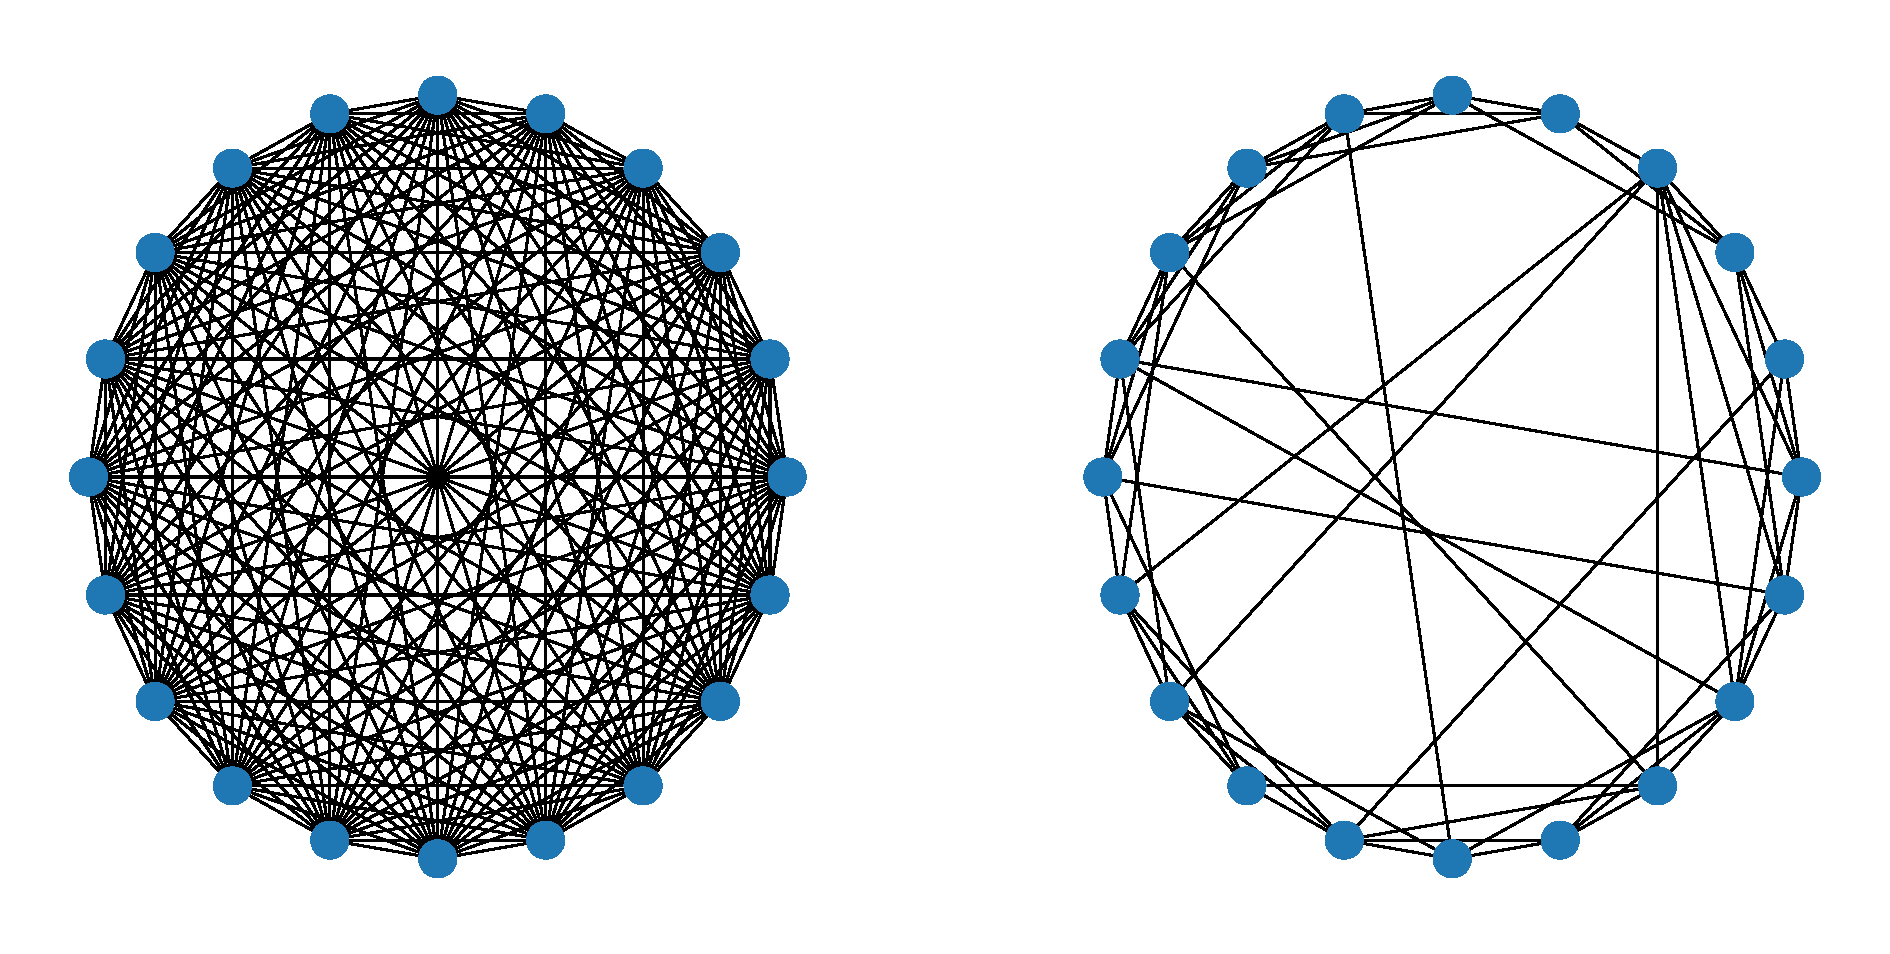
\includegraphics[width=\textwidth]{figs/small_world_all_comparison.pdf}
    \caption{Comparison between the all-to-all network (left) and a small-world network (right) with 20 nodes. 
    The small-world network is constructed from the $k$-nearest neighbour lattice ($k=3$) with the rewriting probability $p=0.2$.}
    \label{fig:all-sw}
  \end{center}
\end{figure}
In this chapter,
we use the Watts--Strogatz small-world network with
$k=3$ and $p=0.2$, following the previous research \cite{hong2002}
which shows emergence of the synchronization transition
on a small-world network.



% In this section, we define the coupled phase-oscillator model on a small-world network,
% and introduce the order parameter to observe synchronization.
% A small-world network possesses the property of a small diameter and a large clustering coefficient
% despite its sparsity.
% This network can be seen in various fields of the real world, such as human relationships,
% World Wide Web, citations of scientific papers, and so on.
% In 1998, Watts and Strogatz proposed a breakthrough network model showing the property of a small-world network,
% which is created in the following algorithm~\cite{watts1998}.
% We first make a periodic $k$-nearest neighbor network with $N$ nodes, which results in $kN$ \blue{links}.
% Then we rewire each \blue{link} with probability $p$,
% keeping in mind that we do not allow self-loops or link duplications.
% \blue{Moreover,} we use only connected small-world networks:
% if a generated network is disconnected,
% we discard it and generate another one until connected one is created.
% See Fig.~\ref{fig:all-sw} for a comparison between the all-to-all network
% and a small-world network.
% \begin{figure}
%   \begin{center}
%     \includegraphics[width=8cm]{mf_sw.eps}
%     \caption{Comparison between the all-to-all network (left) and a small-world network (right) with 20 nodes. 
%     \red{The small-world network is constructed from the $k$-nearest neighbour lattice ($k=3$) with the rewriting probability $p=0.2$.}}
%     \label{fig:all-sw}
%   \end{center}
% \end{figure}
% In this chapter,
% \blue{we use the Watts--Strogatz small-world network with}
% $k=3$ and $p=0.2$, following the previous research
% on the coupled phase-oscillator model on a  small-world network~\cite{hong2002}.

% We consider the coupled phase-oscillator model with $N$ oscillators
% on a small-world network,
% which evolves in time with the following equations,
% \begin{equation}
%   \begin{split}
%     &\frac{\diff\theta_{i}}{\diff t}=\omega_{i}+\frac{K}{2k}\sum_{j\in\Lambda_{i}}f_{a}(\theta_{j}-\theta_{i}),\\
%     &f_{a}(\theta)=\sin\theta+a\sin2\theta,
%     \label{eq:sw-model}
%   \end{split}
% \end{equation}
% for $i=1,\cdots,N$.
% $\theta_{i}$ and $\omega_{i}$ are the phase and the natural frequency of the $i$th oscillator respectively,
% and $\omega_{i}$ is randomly drawn from a natural frequency distribution $g(\omega)$.
% $K>0$ is a coupling constant,
% describing how strong the coupling between oscillators are.
% $\Lambda_{i}$ is the index set, which contains the indexes of oscillators
% connecting to the $i$th oscillator.
% For each oscillator,
% the average number of \blue{links} is $2k$, and we normalize the coupling term by $2k$.
% The coupling function is $f_{a}(\theta)$, and when $a=0$,
% this model is identical to the one proposed in~\cite{hong2002}.

As the natural frequency distribution $g(\omega)$,
we introduce a family of distributions
parametrized by a natural number $n\in\mathbb{N}$,
\begin{align}
  g_{n}(\omega)=\frac{n}{\Gamma(1/(2n))\Delta}e^{-(\omega/\Delta)^{2n}},
  \label{eq:g_n}
\end{align}
where $\Gamma(z)=\int_{0}^{\infty}t^{z-1}e^{-t}\diff t$ is the Gamma function defined on $\Re(z)>0$.
Here, $\Delta>0$ is a parameter describing the width of the distribution. 
We note that $n=1$ gives the Gaussian distribution.
The distribution $g_{n}(\omega)$
is unimodal and symmetric with respect to $\omega=0$,
and its Maclaurin expansion has the following form,
\begin{align}
  g_{n}(\omega)=g_{n}(0)-C_{n}\omega^{2n}+\cdots,
  \label{eq:maclaurin}
\end{align}
where $C_{n}=n/(\Gamma(1/(2n))\Delta^{2n+1})$ is positive.
We remark that the generalized Lorentzian distribution introduced in \cite{pietras2018} also has the same expansion form
up to the second leading term.
In the limit $n\to\infty$, $g_{n}(\omega)$ converges to $g_{\infty}(\omega)$ in the $L^{1}$-norm,
\begin{align}
  g_{\infty}(\omega)=\left\{
  \begin{array}{ll}
    1/(2\Delta), & \omega\in(-\Delta,\Delta),\\
    0, & \mathrm{otherwise}.
  \end{array}
  \right.
\end{align}
This distribution is a uniform distribution on a compact support.
% See Fig.~\ref{fig:g_n} for the graphs of the distributions $g_{n}(\omega)$
% and convergence to $g_{\infty}(\omega)$.
% \begin{figure}
%   \begin{center}
%     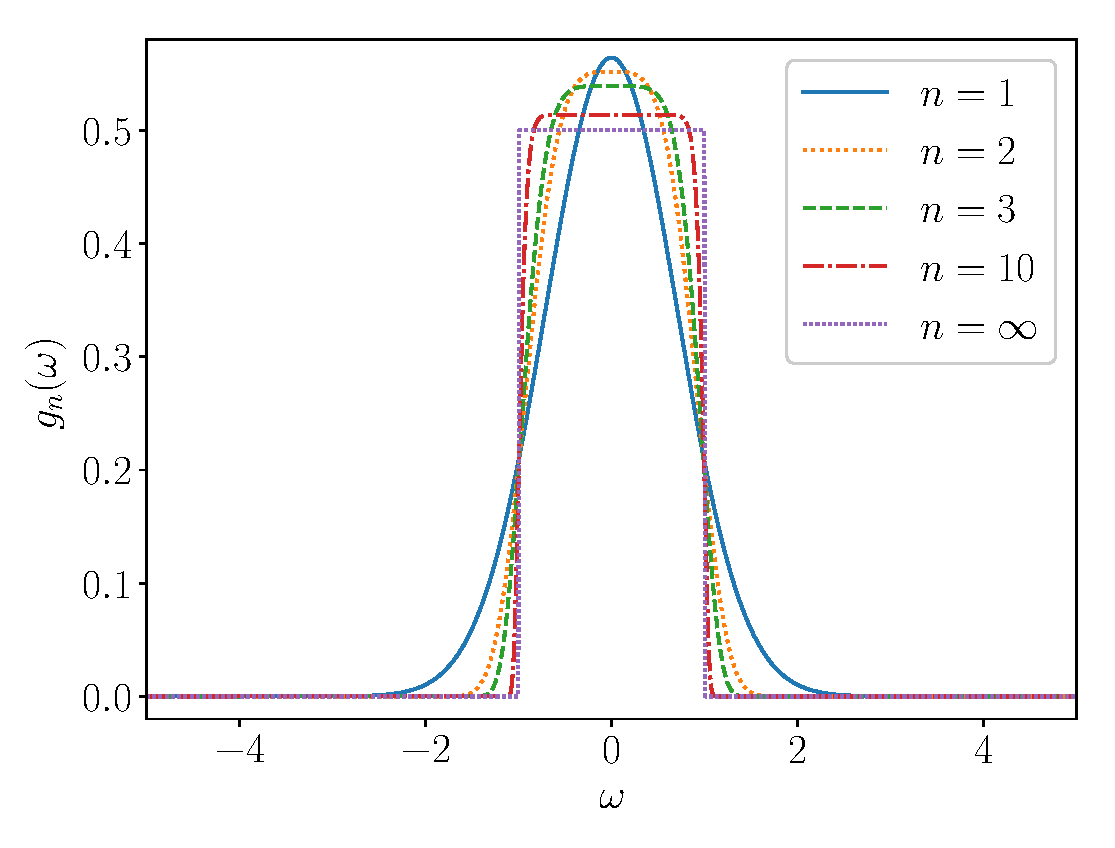
\includegraphics[width=8cm]{figs/gauss_n.eps}
%     \caption{Graphs of $g_{n}(\omega)$ with $n=1,2,3,10,$ and $\infty$,
%     where we set $\Delta=1$.
%     $g_{n}(\omega)$ converges to $g_{\infty}(\omega)$
%     in the limit $n\to\infty$.
    %as $n$ becomes larger.
%     }
%     \label{fig:g_n}
%   \end{center}
% \end{figure}

To visualize the extent of synchronization of oscillators,
we introduce the order parameter $r_{N}$ defined by
% for each coupling strength $K$,
\begin{equation}
  \label{eq:order-parameter}
  r_{N}=\left|\frac{1}{N}\sum_{j=1}^{N}e^{i\theta_{j}}\right|.
\end{equation}
The order parameter represents the centroid of the oscillators moving on the complex unit circle $\mathbb{S}^{1}$.
When the oscillators are uniformly distributed on $\mathbb{S}^{1}$,
which corresponds to the non-synchronized state, $r_{N}$ gets close to 0.
On the other hand, when the oscillators gather at a point on $\mathbb{S}^{1}$,
which corresponds to the synchronized state, $r_{N}$ equals to 1.
The order parameter $r_{N}$ is therefore useful for monitoring synchronization of the coupled phase-oscillator models.
In the next section,
we will look into the dependency of the order parameter $r_{N}$
on the coupling strength $K$.

% We remark a difference between the model considered in \cite{chiba2018,medvedev2014} and ours.
% In the literature,
% the authors consider the coupled phase-oscillator models on the small-world network
% with the equivalent equations as (\ref{eq:sw-model}),
% but they construct the small-world network with each node
% connected to $k=\lfloor sN\rfloor$ neighbors for $s\in(0,0.5)$,
% whereas $k$ is constant regardless of $N$ in our model.
% Here, $\lfloor x\rfloor$ is the floor function that takes the greatest integer less than or equal to $x$.
% As a result, their network has $O(N^{2})$ \blue{links},
% and is much more dense than our network, which has $O(N)$ \blue{links}.
% An advantage of their model is that it can be analyzed through the equation of continuity
% using the graphon~\cite{laszlo2012},
% the continuous limit of the matrix representing the couplings,
% of the small-world network.
%See Fig.~\ref{fig:graphon} for the comparison between the small-world networks
%of \cite{chiba2018,medvedev2014} and ours.
%\begin{figure}
%  \begin{center}
%    \includegraphics[width=8cm]{graphon1.eps}
%  \end{center}
%  \caption{
%    Pixel pictures of the adjency matrix,
%    constructed by turning one to black and zero to white, and scaling to the unit square $[0,1]^{2}$.
%    (Upper row) Pixel pictures of the Watts--Strogatz's small-world networks with $k=10$ and $p=0.2$.
%    (Lower row) Pixel pictures of small-world network, proposed in \cite{chiba2018,medvedev2014}
%    with $k=0.2N$ and $p=0.2$.
%  }
%  \label{fig:graphon}
%\end{figure}

The coupled phase-oscillator model on the small-world network
represented by Eq.~\eqref{eq:sw-model} has been considered previously
\cite{chiba2018,medvedev2014},
but we stress that the numbers of links are completely different from ours.
From the construction algorithm, a small-world network has $kN$ links
and $k=3$ in our networks while $k=O(N)$ in the literature.
An advantage of networks with $k=O(N)$ is that they can be analyzed
through the equation of continuity \cite{laszlo2012}.
Nevertheless, this advantage implies at the same time
that such a small-world network in the literature
is essentially the same with the all-to-all coupling,
and is not suitable for detecting new universality classes.

% \blue{(この段落の内容は前に言っているのでまるごと削除)}
% We note the dependency on $p$ for a synchronization transition.
% For $p=0$, the small-world network becomes the periodic one-dimensional $k$-nearest-neighbor network.
% In \cite{hong2002},
% the authors numerically showed that a coupled phase-oscillator model on a $k$-nearest-neighbor network
% does not show a synchronization transition;
% $r\approx0$ for all $K$.
% However, if $p$ is greater than zero,
% a synchronization transition occurs because of emergence of shortcuts.

\section{Numerical simulations}
\label{sec:nu-sim}
In the large population limit $N\to\infty$,
the coupled phase-oscillator model, Eq.~(\ref{eq:sw-model}), is
expected to show a synchronization transition around a critical point $K_{\mathrm{c}}$.
For $K<K_{\mathrm{c}}$, the order parameter $r(K):=\lim_{N\to\infty}r_{N}(K)$ is zero,
which corresponds to the non-synchronized state.
On the other hand, for $K>K_{\mathrm{c}}$,
the model shows partially synchronized states, in which $r(K)$ exhibits power law behavior close to the critical point
in the form of
\begin{align}
  r(K)\sim(K-K_{\mathrm{c}})^{\beta},
\end{align}
where $\beta$ is one of the critical exponents.
The critical exponents are crucial to describe critical phenomena,
and models are classified into universality classes, each of which shares the same critical exponents.
Calculating the critical exponents, including $\beta$, is therefore
an important topic from theoretical and numerical perspectives.
% In this section, we numerically calculate the critical exponent $\beta$ of the coupled phase-oscillator models
% on small-world networks.

% The critical exponent $\beta$ is defined in the large population limit $N\to\infty$,
% and this cannot be achieved through the numerical simulations.
% %To overcome this difficulty,
% %we use the finite-size scaling,
% %that is, we assume that there exists a function $F$, so called the scaling function,
% %and that the order parameter reads
% %\begin{align}
% %r_{N}(K)=N^{-\beta/\bar{\nu}}F((K-K_{\mathrm{c}})N^{1/\bar{\nu}}).
% %\label{eq:finite-size}
% %\end{align}
% %Here, the critical exponent $\bar{\nu}$ is defined through the correlation length $\xi$, which diverges at $K=K_{\mathrm{c}}$ with
% %\begin{align}
% %\xi\propto(K-K_{\mathrm{c}})^{-\bar{\nu}}.
% %\end{align}
% \red{
% To overcome this difficuty, we discuss the finite-size scaling theory.
% In lattice models, the correlation length $\xi$ plays an important role in the finite-size scaling,
% but it cannot be defined in the systems with oscilators on a small-world network.
% Instead we introduce the conherent number $N_{\mathrm{c}}$~\cite{botet1982},
% which is assumed to diverge at $K=K_{\mathrm{c}}$ with
% \begin{align}
% N_{\mathrm{c}}\propto(K-K_{\mathrm{c}})^{\bar{\nu}},
% \end{align}
% as $N\to\infty$.
% Using $\bar{\nu}$, the scaling function for $r_{N}(K)$, denoted by $F$, can be introduced as
% \begin{align}
% r_{N}(K)=N^{-\beta/\bar{\nu}}F((K-K_{\mathrm{c}})N^{1/\bar{\nu}}).
% \label{eq:finite-size}
% \end{align}
% }
% The finite-size scaling is widely used for numerical studies
% of critical phenomena in second-order phase transitions,
% including coupled phase-oscillator models~~\cite{pelisseto2002,hasenbusch2010,pikovsky2015,hong2002,hong2015,coletta2017,juhasz2019}.
% In this chapter, we use a new statistical method \red{called the Bayesian scaling analysis}~\cite{harada2011,harada2015}
% to estimate the values of $K_{\mathrm{c}}, \beta$ and $\bar{\nu}$ in the finite-size scaling relation.
% Using a new technique in the field of machine learning, 
% we can automatically find the best parameter set with a good collapse of data points 
% onto a scaling function $F$.
% \red{
% See Appendix \ref{sec:bsa} for a brief introduction to the Bayesian scaling analysis.
% }


\subsection{Finite-size scaling}
The critical exponent $\beta$ is defined in the large population limit
$N\to\infty$, but the limit cannot be achieved through the numerical
simulations. To overcome this difficulty, we use the finite-size
scaling theory, which provides us the limit from observations
in finite-size systems.
The first assumption of our finite-size scaling theory is
existence of the coherent number $N_{\rm c}(K)$ \cite{botet1982} diverging at
the critical point $K=K_{\rm c}$ as
\begin{equation}
  N_{\rm c}(K) \propto (K-K_{\rm c})^{-\bar{\nu}},
\end{equation}
where $\bar{\nu}$ is another unknown positive critical exponent.
The coherent number corresponds to the correlation length
in a simple lattice model.
The second assumption is that the order parameter $r_{N}(K)$
depends on $K$ only through the ratio
\begin{equation}
  \dfrac{N}{N_{\rm c}(K)} \propto \left[ (K-K_{\rm c})N^{1/\bar{\nu}} \right]^{\bar{\nu}}.
\end{equation}
These assumptions imply that $r_{N}(K)$ can be represented by
\begin{equation}
  \label{eq:finite-size}
  r_{N}(K) = N^{-\beta/\bar{\nu}} F((K-K_{\rm c})N^{1/\bar{\nu}}),
\end{equation}
where the function $F$, which is called the scaling function, must be
\begin{equation}
  F(x) \propto x^{\beta} \quad \text{for large } x
\end{equation}
to reproduce the critical exponent $\beta$ in the limit $N\to\infty$.
We remark that the exponent $\beta/\bar{\nu}$ expresses
the finite-size fluctuation of $r_{N}(K)$
at the critical point $K=K_{\rm c}$.

The finite-size scaling is widely used for numerical studies
of critical phenomena in continuous phase transitions,
including coupled phase-oscillator models \cite{hong2002,pelissetto2002,hasenbusch2010,pikovsky2015,hong2015,coletta2017,juhasz2019}.
An important remark on Eq.~\eqref{eq:finite-size} is that,
on the $((K-K_{\rm c})N^{1/\bar{\nu}}, N^{\beta/\bar{\nu}}r_{N})$ plane,
observed values of $r_{N}(K)$ must collapse on a single graph of $F$
for any values of $N$ and $K$.
The unknown values of $K_{\rm c}, \beta$, and $\bar{\nu}$
are determined by detecting the best fit values.
The detection will be performed by using the Bayesian scaling analysis
\cite{harada2011,harada2015},
whose brief introduction is given in Appendix \ref{sec:bsa}.


\subsection{Computation of the order parameter}

We determine the value of the order parameter $r_{N}(K)$
for a given set of $(N,K)$
through temporal evolution of the system and
two steps of averaging.
The model equation, Eq.~\eqref{eq:sw-model},
is numerically integrated by using the fourth-order Runge--Kutta algorithm
with the time step $\delta t=0.1$.
Initial values of the phases $\{\theta_{i}\}$
are randomly drawn from the uniform distribution on the interval $[0,2\pi)$,
and the natural frequencies $\{\omega_{i}\}$ are randomly drawn
from the distribution function $g_{n}(\omega)$.
The order parameter $r_{N}$ defined by Eq.~\eqref{eq:order-parameter}
depends on time $t$,
and we take the time average in the time interval $t\in [300,500]$.
This is the first averaging.
% Further, we perform $400$ realizations by changing small-world networks,
% the initial values of $\{\theta_{i}\}$ and $\{\omega_{i}\}$
% for a given set of $(N,K)$.

Further, we perform $400$ realizations by changing small-world networks,
the initial values of $\{\theta_{i}\}$, and $\{\omega_{i}\}$
for a given set of $(N,K)$.
To compute the confidence interval of the order parameter,
the resampling technique is in use.
We choose $200$ samples out of $400$ realizations,
and calculate the mean of the time-averaged order parameter
in the chosen $200$ samples.
The mean of the $i$th resampling is denoted by $r_{N}^{(i)}(K)$,
and we perform the resampling for $S=1000$ times.
The value $r_{N}(K)$ is determined by taking the second averaging
over $S$ samples $\{r_{N}^{(i)}(K)\}_{i=1}^{S}$,
which also provide the confidence interval of $r_{N}(K)$.


See Fig.~\ref{fig:bif-fss} for the obtained $r_{N}(K)$ for $a=0$ and $-0.2$ with $n=1$,
where the condition $a\leq 0$ is expected to give a continuous transition.
In the following two sections, we compute the critical exponents
for $a=0$ and $a=-0.2$,
and show discontinuity for $a=0.5$, respectively.
We remark that $a=-0.2$ and $0.5$ are not special values.
They are arbitrarily chosen from a neighborhood of $a=0$ to demonstrate
differences among the three cases of (i) $a=0$, (ii) $a<0$, and (iii) $a>0$.



% Numerical simulations of the coupled phase-oscillator model on the small-world networks
% are performed by using the fourth-order Runge--Kutta algorithm
% with the time step $\delta t=0.1$.
% We first make a Watts--Strogatz's small-world network, and for each $K$, 
% we numerically integrate \blue{Eq.~(\ref{eq:sw-model})}
% by setting random initial phases and random natural frequencies obeying $g_{n}(\omega)$,
% and we take the time average of the order parameter in the time interval $t\in[300,500]$.
% We performed 400 realizations by changing small-world networks,
% \blue{the initial values of $\theta_{i}$'s, and $\omega_{i}$
%   for a given set of $(N,K)$.}
% %for each system size, which we take from $N=1600$ to $N=25600$.
% The order parameter $r_{N}(K)$ and its errorbar are evaluated by the resampling technique:
% We randomly choose 200 samples out of 400 realizations,
% % and we calculate the mean of the order parameter,
% % which we refer to $\{r_{N}^{(i)}(K)\}_{i=1}^{S}$.
% % We take this step for $S=1000$ times, and 
% % $r_{N}(K)$ is given by the mean of $\{r_{N}^{(i)}(K)\}_{i=1}^{S}$,
% % and the confidence interval of $r_{N}(K)$ is given by the statistical deviation of $\{r_{N}^{(i)}(K)\}_{i=1}^{S}$.
% % We will show results of $a=0, -0.2$, and $0.5$, chosen from the neighborhood of $a=0$,
% % as the case (i), (ii), and (iii), respectively.
% % The order of the second-leading term in the natural frequency distribution
% % are taken as $n= 1, 2, 3$, and $\infty$.
% % See Fig.~\ref{fig:bif-fss} for the numerical results with $n=1$ and $a=0,-0.2$.
% \blue{
%   and calculate the mean of the time-averaged order parameter
%   in the choosen $200$ samples.
% The sampling is performed $S=1000$ times,
% and the mean for the $i$th sampling is denoted by $\overline{r}_{N}^{(i)}(K)$.
% The value of the order parameter $r_{N}(K)$
% is defined as the average over $\{\overline{r}_{N}^{(i)}(K)\}_{i=1}^{S}$,
% and the $S$ sample values also give the confidence interval of $r_{N}(K)$.
% See Fig.3 for the obtained $r_{N}(K)$ for $a=0$ and $-0.2$
% with $n=1,2,3$, and $\infty$.
% }


\subsection{Critical exponents for continuous transition}

\begin{figure}[t]
  \begin{center}
    % 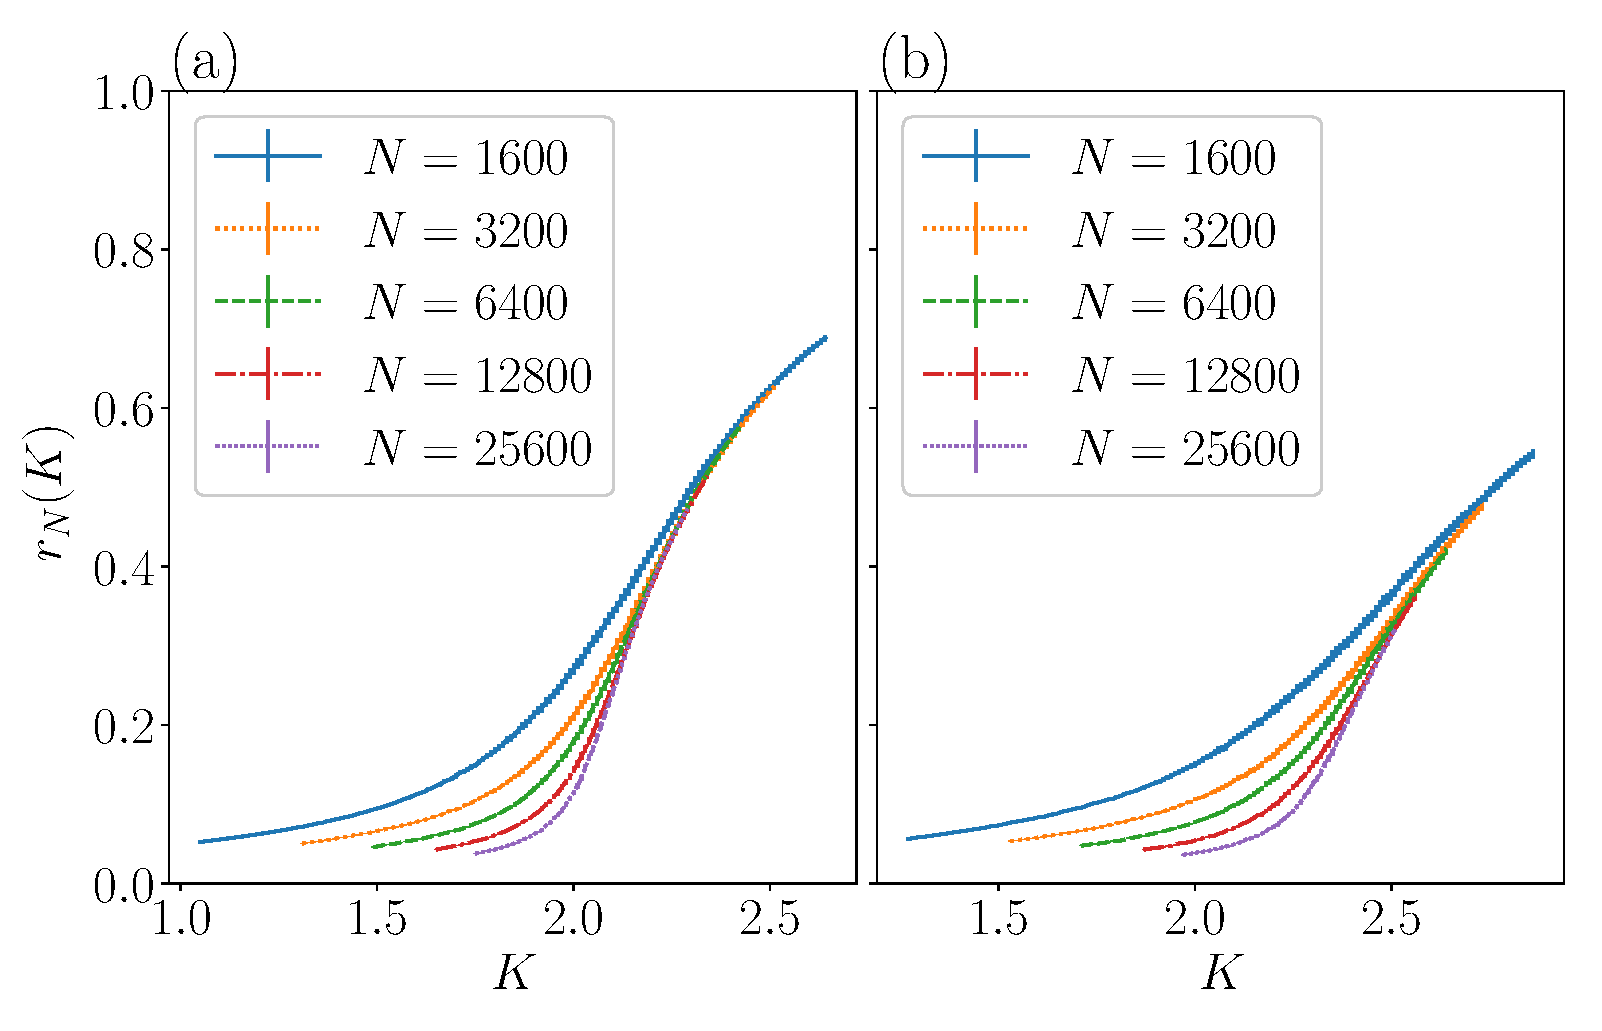
\includegraphics[width=\textwidth]{figs/bif-fss-all.eps}
    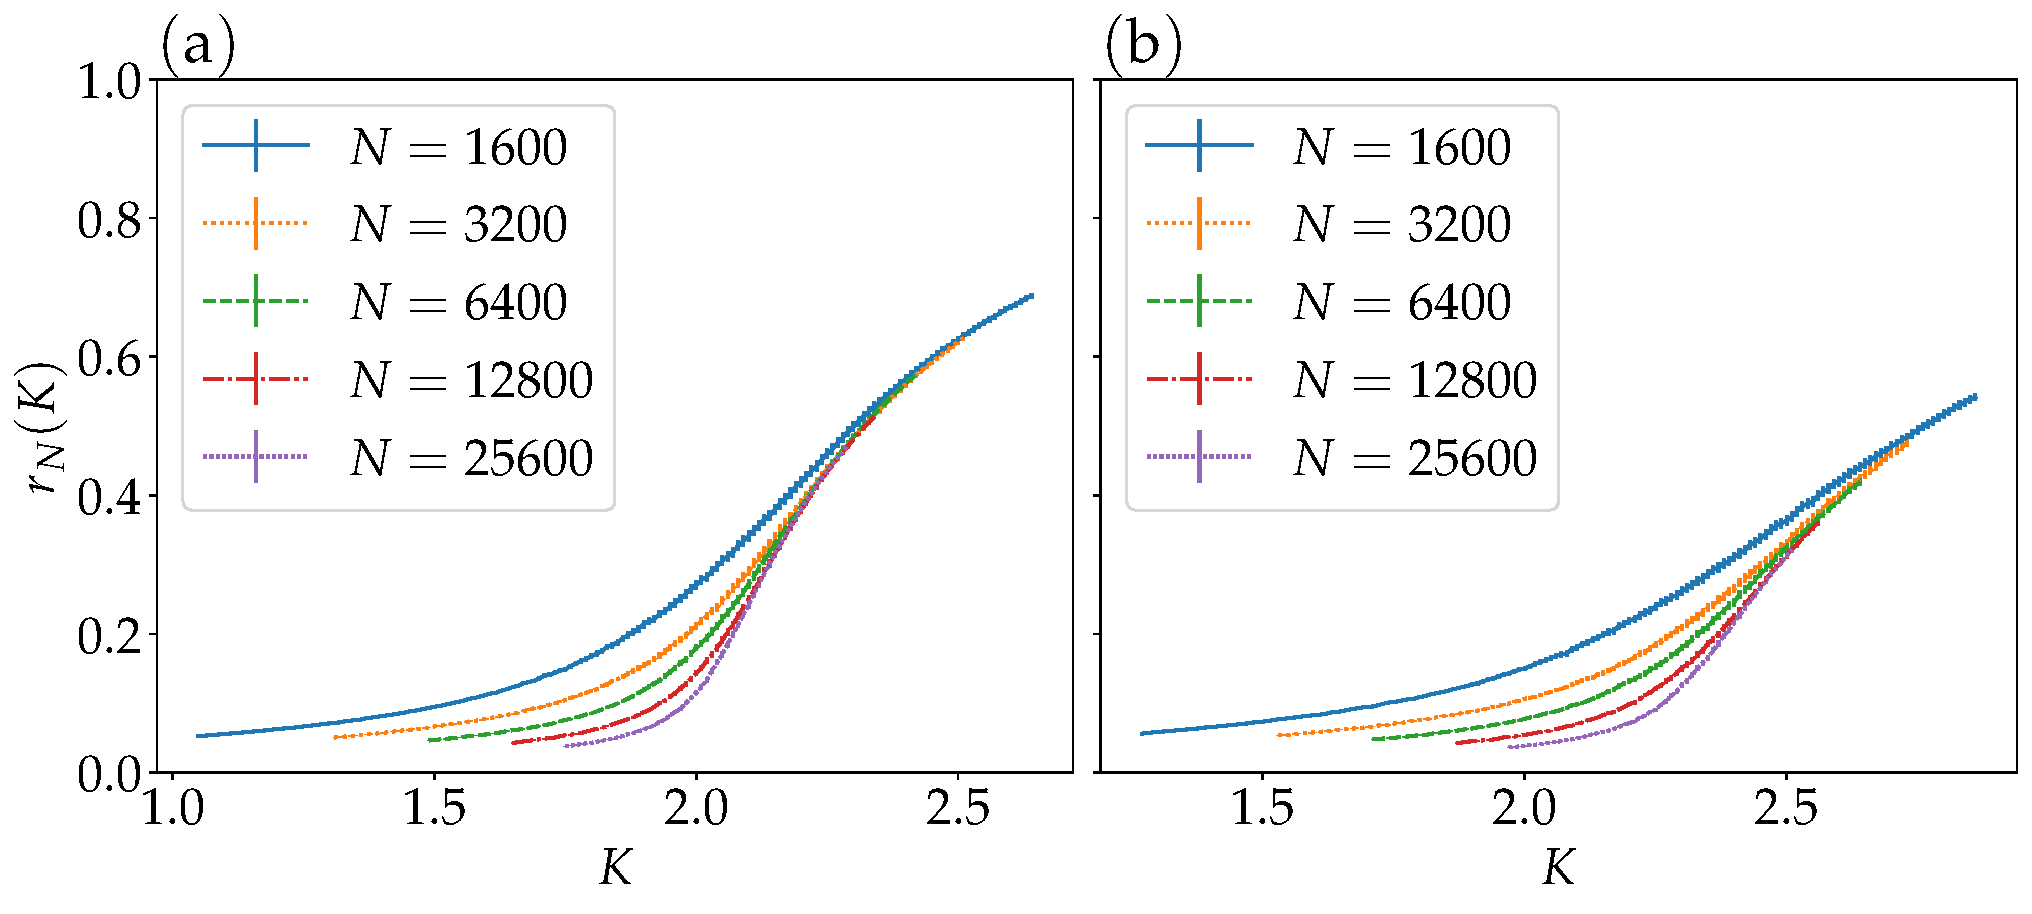
\includegraphics[width=\textwidth]{figs/small_world_orderparam.pdf}
  \end{center}
  \caption{
    Graphs of order parameter $r_{N}(K)$ with its confidence interval for the model \eqref{eq:sw-model},
    where we take the coupling function $f_{a}(\theta)$
    with (a) $a=0$ and (b) $a=-0.2$.
    As a natural frequency distribution,
    we use $g_{1}(\omega)$ with $\Delta=1$,
    and $N=1600, 3200, 6400, 12800,$ and $25600$ from top to bottom.
    $r_{N}(K)$ and its confidence interval are evaluated by the resampling technique.
    Errorbars are so small that they may not be visible.
  }
  \label{fig:bif-fss}
\end{figure}


% Once we obtain $r_{N}(K)$ for several system size $N$,
% we evaluate the critical exponents $\beta$ and $\bar{\nu}$ and the critical point $K_{\mathrm{c}}$
% from the scaling relation (\ref{eq:finite-size}).
% We determine these values by finding the best values so that points of $r_{N}(K)N^{\beta/\bar{\nu}}$
% as a function of $(K-K_{\mathrm{c}})N^{1/\bar{\nu}}$
% are tightly collapsed to a scaling function $F$.
% Here we again use the resampling method to obtain the critical exponents and their confidence intervals:
% By introducing the symbol $N_{\min}$ to indicate the smallest system size for the finite-size scaling analysis,
% we use $r_{N_{\min}}^{(i)}(K),r_{2\cdot N_{\min}}^{(i)}(K)$, and $r_{4\cdot N_{\min}}^{(i)}(K)$
% to evaluate $\beta,\bar{\nu}$, and $K_{\mathrm{c}}$ by the Bayesian scaling analysis~\cite{harada2011,harada2015}.
% \red{
% We use different subsets of the data by varying $N_{\min}$,
% and expect the estimated values to converge to a true value as $N_{\min}$ increases.
% }
% Figure \ref{fig:scatter} shows $\beta, \nu$, and $K_{\mathrm{c}}$ estimated from each resampling data set.
% Mean values and standard deviations of $\beta,\bar{\nu}$, and $K_{\mathrm{c}}$
% give us the best-fit parameters and confidence intervals.
% We carried out this procedure for $N_{\min}=1600,3200$, and $6400$\red{, and confirmed that the data are collapsed to a scaling function for each $N_{\min}$.}
% The graph of $r_{N}(K)N^{\beta/\bar{\nu}}$ versus $(K-K_{\mathrm{c}})N^{1/\bar{\nu}}$
% are shown in Fig.~\ref{fig:fit} for checking the validity of the estimated parameters $\beta,\bar{\nu}$, and $K_{\mathrm{c}}$ \red{at $N_{\min}=6400$}.

\begin{figure}[t]
  \begin{center}
    % 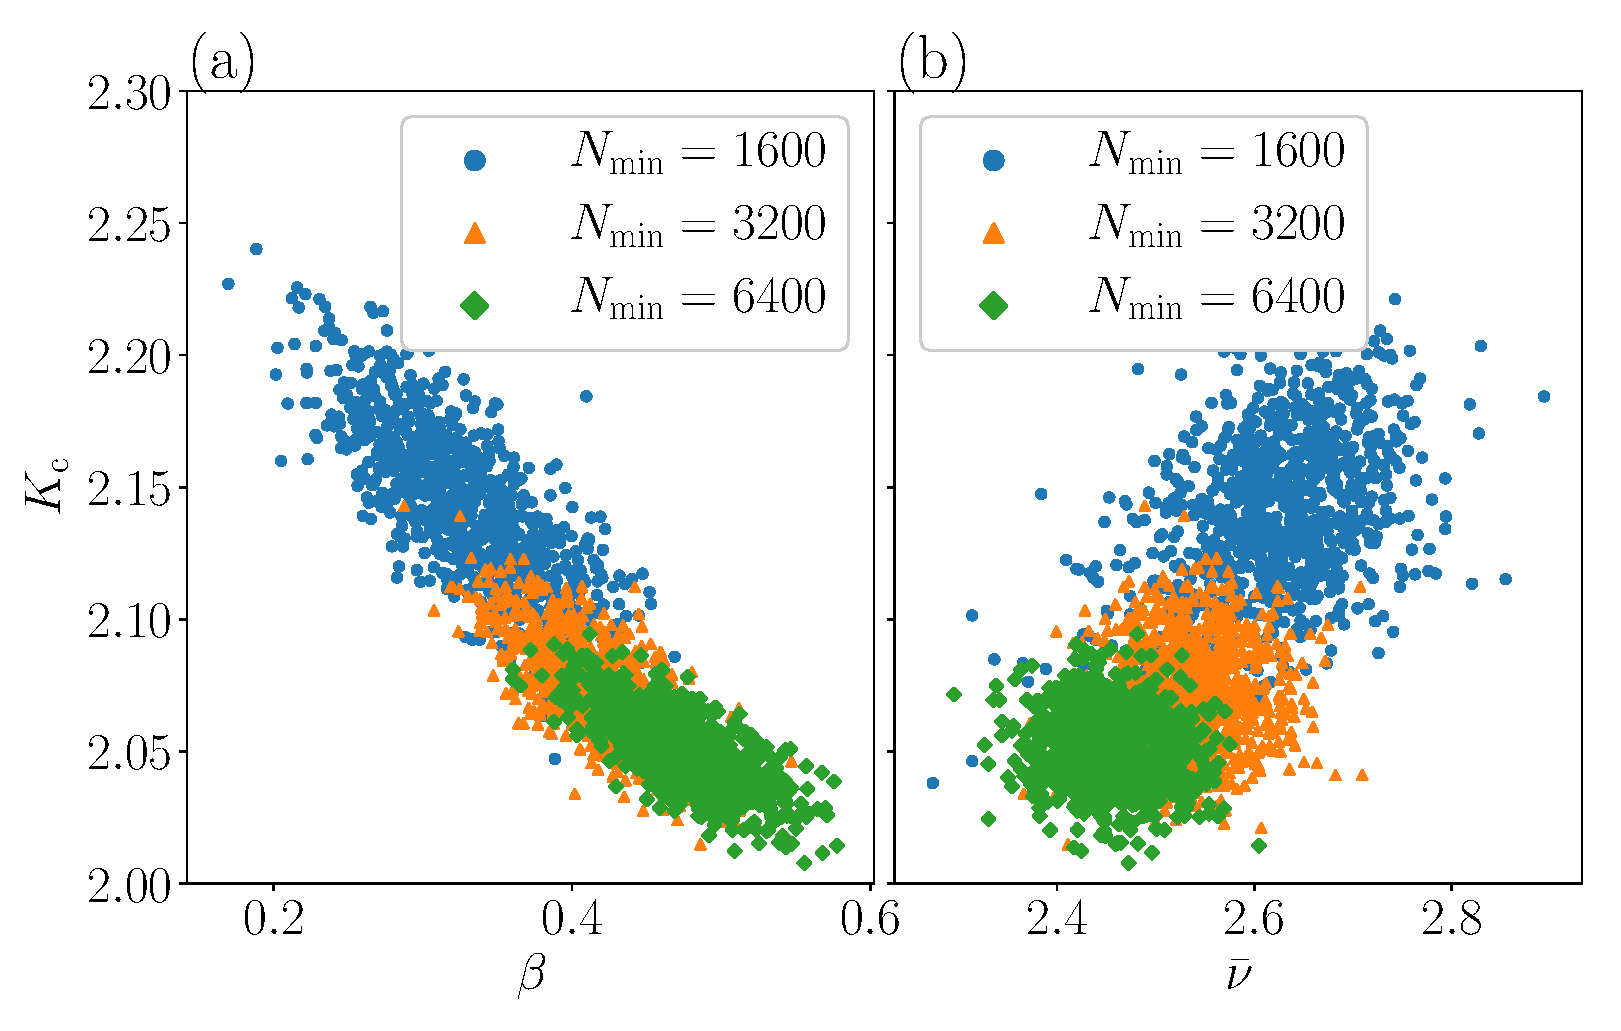
\includegraphics[width=\textwidth]{figs/scatter.eps}
    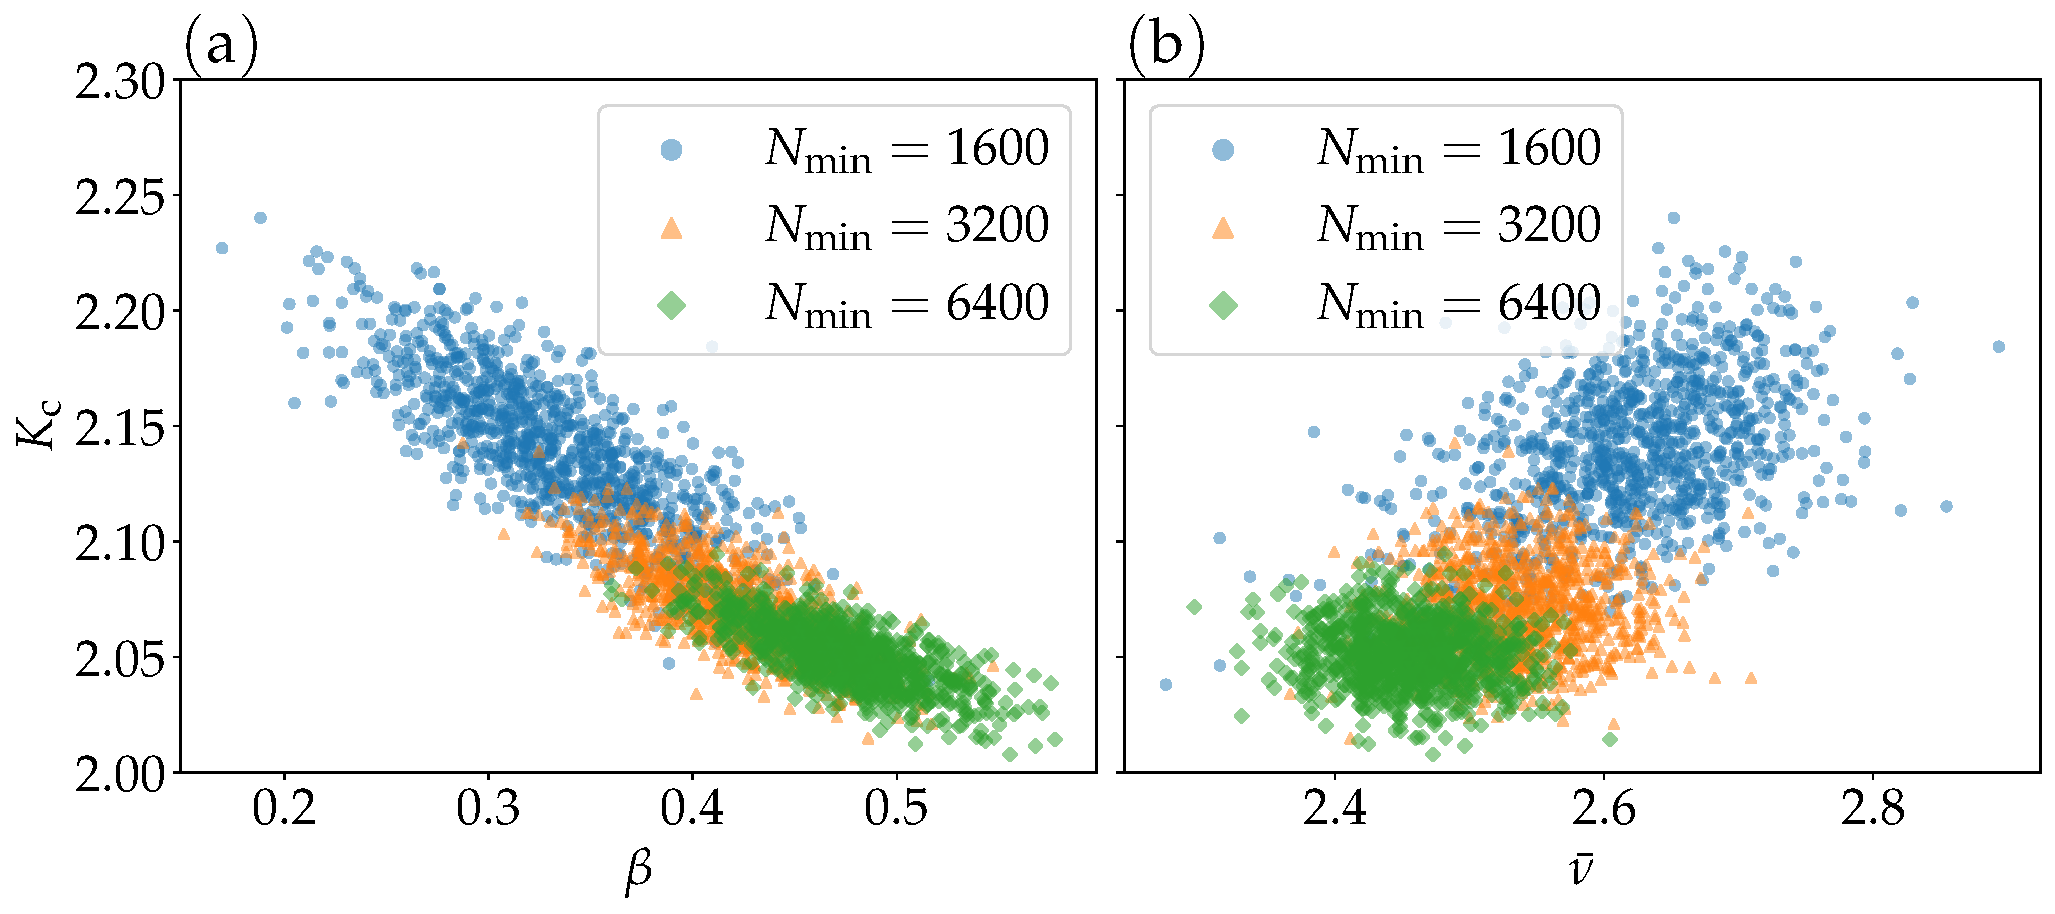
\includegraphics[width=\textwidth]{figs/critical_val_scatter.pdf}
  \end{center}
  \caption{
    Scattering plots of computed parameters (a)$(\beta,K_{\mathrm{c}})$ and (b)$(\bar{\nu},K_{\mathrm{c}})$, 
    evaluated by the Bayesian scaling analysis.
    Here, we use $(a,n)=(0,1)$, and we set $N_{\min}$ to $1600,3200$ and $6400$.
  }
  \label{fig:scatter}
\end{figure}

The finite-size scaling, Eq.~\eqref{eq:finite-size}, is
a powerful tool to compute the unknown values of
$K_{\rm c},\beta$, and $\bar{\nu}$,
but it is not perfect if $N$ is not sufficiently large.
We thus compute the unknown variables
for three values of $N\in\{N_{\rm min},~ 2N_{\rm min}, ~4N_{\rm min}\}$,
and observe convergence by varying $N_{\rm min}$.
% More precisely, the unknown values are computed
% throught the finite-size scaling
% for the sets of $N\in\{1600, 3200, 6400\}$,
% $\{3200, 6400, 12800\}$, and $\{6400, 12800, 25600\}$.
Moreover, we use the resampling technique again
to estimate the unknown values with their confidence intervals.
Consequently, we have $S=1000$ sets of the three values
for a given $N_{\rm min}$ as reported in Fig.~\ref{fig:scatter}
because each resampling set $r_{N}^{(i)}(K)$ determines them.
Finally, the values and the confidence intervals
of $K_{\rm c},\beta$, and $\bar{\nu}$
are computed as the averages and the standard deviations
over $S=1000$ sets.
The estimated values are verified in Fig.~\ref{fig:fit},
where all the points lie on a single curve representing
the scaling function $F$ for $N_{\rm min}=6400$.


\begin{figure}[t]
  \begin{center}
    % 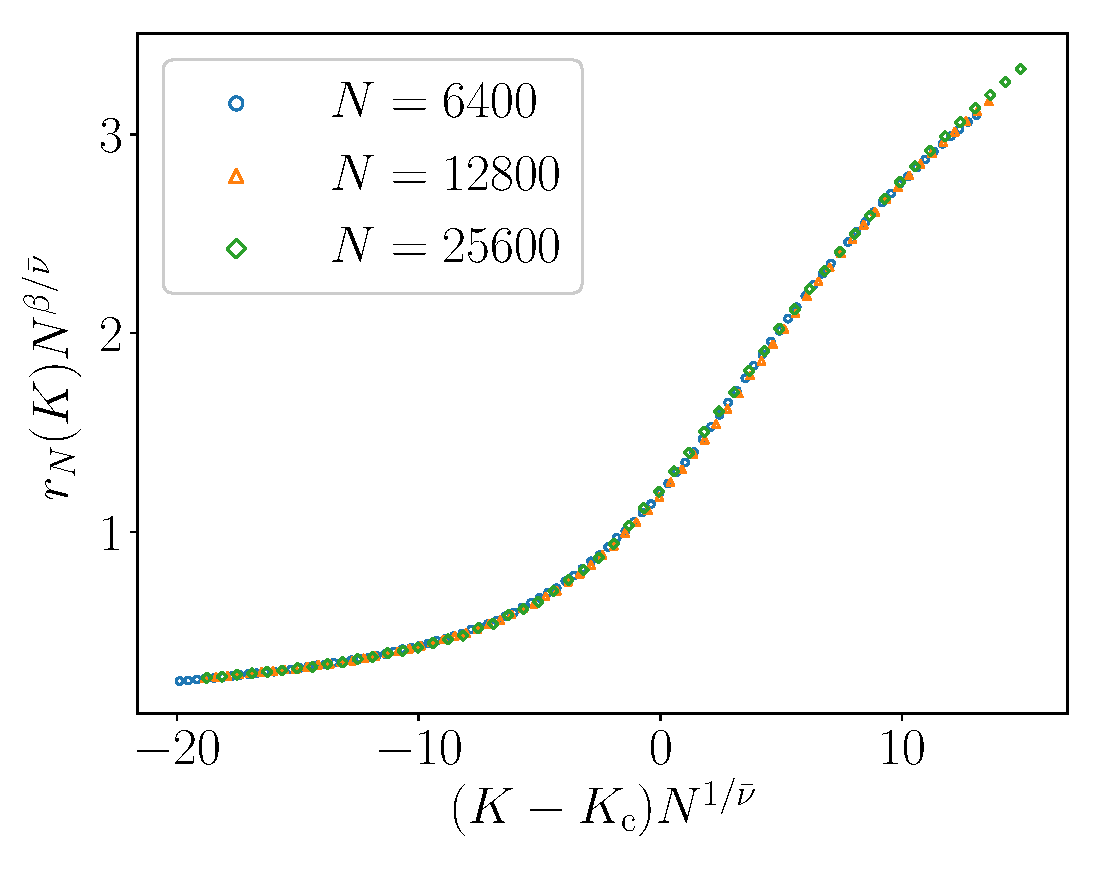
\includegraphics[width=8cm]{figs/fit.eps}
    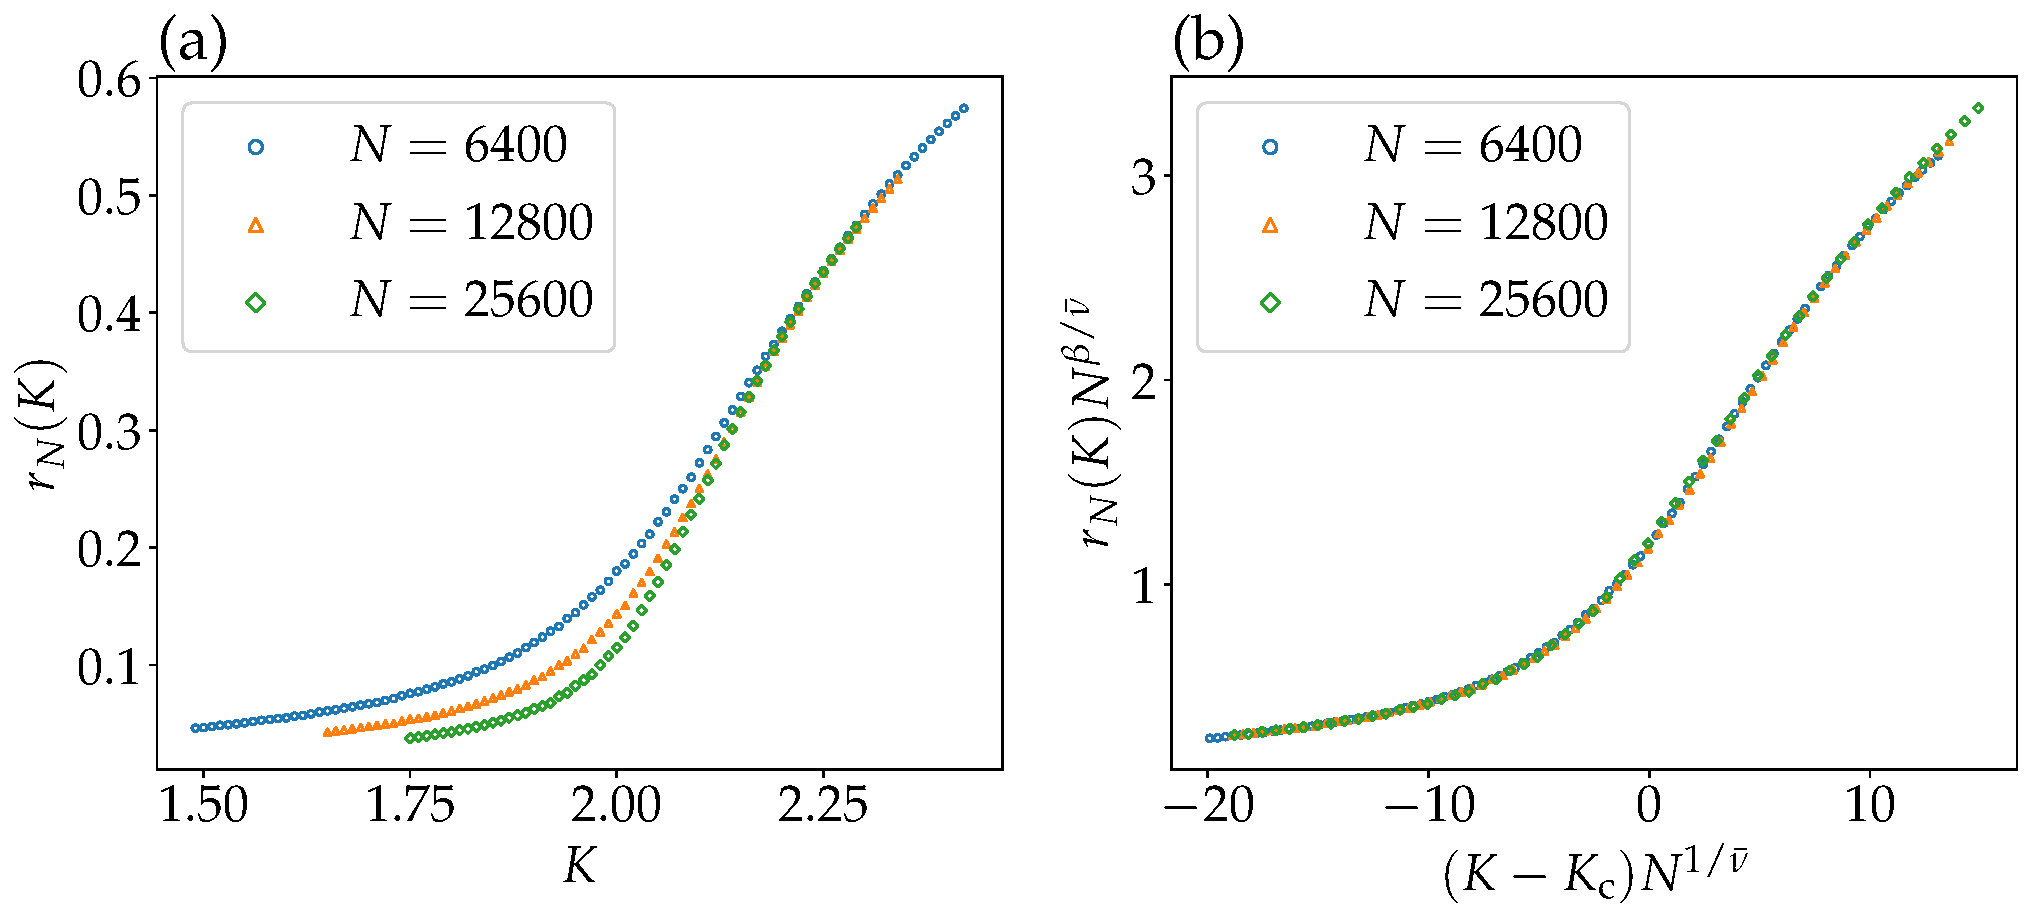
\includegraphics[width=\textwidth]{figs/collapse_plot.pdf}
  \end{center}
  \caption{
    Graph of scaled order parameter $r_{N}(K)N^{\beta/\bar{\nu}}$ versus scaled coupling constant $(K-K_{\mathrm{c}})N^{1/\bar{\nu}}$
    for $(a,n)=(0,1)$,
    where we use $\beta,\bar{\nu}$ and $K_{\mathrm{c}}$, obtained by the Bayesian scaling analysis for $N_{\min}=6400$.
    The values of $\beta,\ \bar{\nu}$, and $K_{\mathrm{c}}$ are shown in Table \ref{table:parameter-estimate}.
    We see that the scaled data are well collapsed to the scaling function $F$.
  }
  \label{fig:fit}
\end{figure}


\begin{table*}[t]
  \begin{center}
    \caption{Critical exponents $\beta,\bar{\nu}$ and the critical point $K_{\mathrm{c}}$ of \eqref{eq:sw-model} depending on the coupling function $f_{a}(\theta)=\sin\theta+a\sin2\theta$ and the natural frequency distribution $g_{n}(\omega)$ in \eqref{eq:g_n}, for $a=0$ and $-0.2$ and $n=1,2,3$, and $\infty$.
    For each pair of $(a,n)$, we use $N_{\min}=1600,3200,6400$, and execute the Bayesian scaling analysis~\cite{harada2011} to find the best parameters fitting \eqref{eq:finite-size}.
    We extrapolate the critical values to $N_{\min}=\infty$ by using the least square method,
    and they are listed in the line of $N_{\min}=\infty$.
    Here, we show the confidence intervals for the last digit of the estimated values 
    in parentheses; for example, $2.13(3)=2.13\pm0.03$.
  }
    \label{table:parameter-estimate}
    \begin{tabular*}{\linewidth}{@{\extracolsep{\fill}}cccccc}\hline
      $f_{a}(\theta)$ & $g_{n}(\omega)$ & $N_{\min}$ & $K_{\mathrm{c}}$ & $\beta$ & $\bar{\nu}$ \\\hline\hline
      $a=0$ & $n=1$ & $1600$ & $2.13(3)$ & $0.33(4)$ & $2.61(7)$ \\
       & & $3200$ & $2.07(1)$ & $0.42(3)$ & $2.53(5)$ \\
       & & $6400$ & $2.05(1)$ & $0.47(3)$ & $2.45(4)$ \\
       & & $\mathbf{\infty}$ & $\mathbf{2.02(2)}$ & $\mathbf{0.51(4)}$ & $\mathbf{2.40(6)}$ \\\cline{2-6}
       & $n=2$ & $1600$ & $1.85(1)$ & $0.27(2)$ & $2.67(5)$\\
       & & $3200$ & $1.78(1)$ & $0.37(2)$ & $2.53(3)$\\
       & & $6400$ & $1.755(9)$ & $0.44(2)$ & $2.50(3)$\\
       & & $\mathbf{\infty}$ & $\mathbf{1.72(1)}$ & $\mathbf{0.49(2)}$ & $\mathbf{2.43(4)}$ \\\cline{2-6}
       & $n=3$ & $1600$ & $1.80(1)$ & $0.28(2)$ & $2.62(4)$\\
       & & $3200$ & $1.76(1)$ & $0.33(2)$ & $2.51(3)$\\
       & & $6400$ & $1.723(8)$ & $0.44(2)$ & $2.51(3)$\\
       & & $\mathbf{\infty}$ & $\mathbf{1.69(1)}$ & $\mathbf{0.47(2)}$ & $\mathbf{2.46(4)}$ \\\cline{2-6}
       & $n=\infty$ & $1600$ & $1.83(1)$ & $0.27(1)$ & $2.50(4)$ \\
       & & $3200$ & $1.79(1)$ & $0.36(2)$ & $2.52(3)$ \\
       & & $6400$ & $1.780(8)$ & $0.41(2)$ & $2.46(3)$ \\
       & & $\mathbf{\infty}$ & $\mathbf{1.76(1)}$ & $\mathbf{0.46(2)}$ & $\mathbf{2.46(4)}$ \\\hline
       $a=-0.2$ & $n=1$ & $1600$ & $2.43(5)$ & $0.38(8)$ & $2.67(9)$ \\
       & & $3200$ & $2.35(2)$ & $0.44(6)$ & $2.58(7)$ \\
       & & $6400$ & $2.34(1)$ & $0.45(4)$ & $2.42(6)$ \\
       & & $\mathbf{\infty}$ & $\mathbf{2.31(3)}$ & $\mathbf{0.48(6)}$ & $\mathbf{2.36(8)}$ \\\cline{2-6}
       & $n=2$ & $1600$ & $2.09(3)$ & $0.31(4)$ & $2.87(7)$\\
       & & $3200$ & $1.99(2)$ & $0.41(4)$ & $2.65(5)$\\
       & & $6400$ & $1.96(1)$ & $0.47(3)$ & $2.52(4)$\\
       & & $\mathbf{\infty}$ & $\mathbf{1.91(2)}$ & $\mathbf{0.51(4)}$ & $\mathbf{2.41(6)}$ \\\cline{2-6}
       & $n=3$ & $1600$ & $2.04(3)$ & $0.27(5)$ & $2.85(8)$\\
       & & $3200$ & $1.96(2)$ & $0.37(4)$ & $2.65(5)$\\
       & & $6400$ & $1.91(1)$ & $0.49(3)$ & $2.59(4)$\\
       & & $\mathbf{\infty}$ & $\mathbf{1.86(2)}$ & $\mathbf{0.55(4)}$ & $\mathbf{2.50(6)}$ \\\cline{2-6}
       & $n=\infty$ & $1600$ & $2.08(3)$ & $0.25(4)$ & $2.76(6)$ \\
       & & $3200$ & $2.00(1)$ & $0.38(4)$ & $2.69(5)$ \\
       & & $6400$ & $1.97(1)$ & $0.43(3)$ & $2.54(4)$ \\
       & & $\mathbf{\infty}$ & $\mathbf{1.94(2)}$ & $\mathbf{0.49(4)}$ & $\mathbf{2.49(6)}$ \\\hline
    \end{tabular*}
  \end{center}
\end{table*}

% Results of the parameters by the Bayesian scaling analysis are summarized
% in Table~\ref{table:parameter-estimate}.
% Here we extrapolate the critical values
% to $N_{\min}=\infty$ by plotting the values of $K_{\mathrm{c}}$, $\beta$ and $\bar{\nu}$ as a function of $1/N_{\min}$,
% and use the least square method to find the values at $\lim_{N_{\min}\to\infty}1/N_{\min}=0$.
% The extrapolated values are listed in the line of $N_{\min}=\infty$ in Table~\ref{table:parameter-estimate}.
% See Fig.~\ref{fig:ce_extrapolation} for the extrapolation of $\beta$ with $a=0$ and $-0.2$.

The estimated values of $K_{\rm c}, \beta$ and $\bar{\nu}$
are summarized in Table~\ref{table:parameter-estimate}.
The row of $N_{\min}=\infty$ is obtained by extrapolation
from $N_{\min}=1600, 3200$, and $6400$
as demonstrated in Fig.~\ref{fig:ce_extrapolation}.
We note that the extrapolated values of $\beta$ are close to $1/2$
and ones of $\bar{\nu}$ are close to $5/2$
irrespective of the values of $a$ and $n$.
The universality is completely unlike the all-to-all interaction case.
Here we note that this result shares the same critical exponent $\bar{\nu}=5/2$
as the all-to-all interaction case for $(a,n)=(0,1)$
calculated in \cite{hong2007}.

\begin{figure}[t]
  \begin{center}
    % 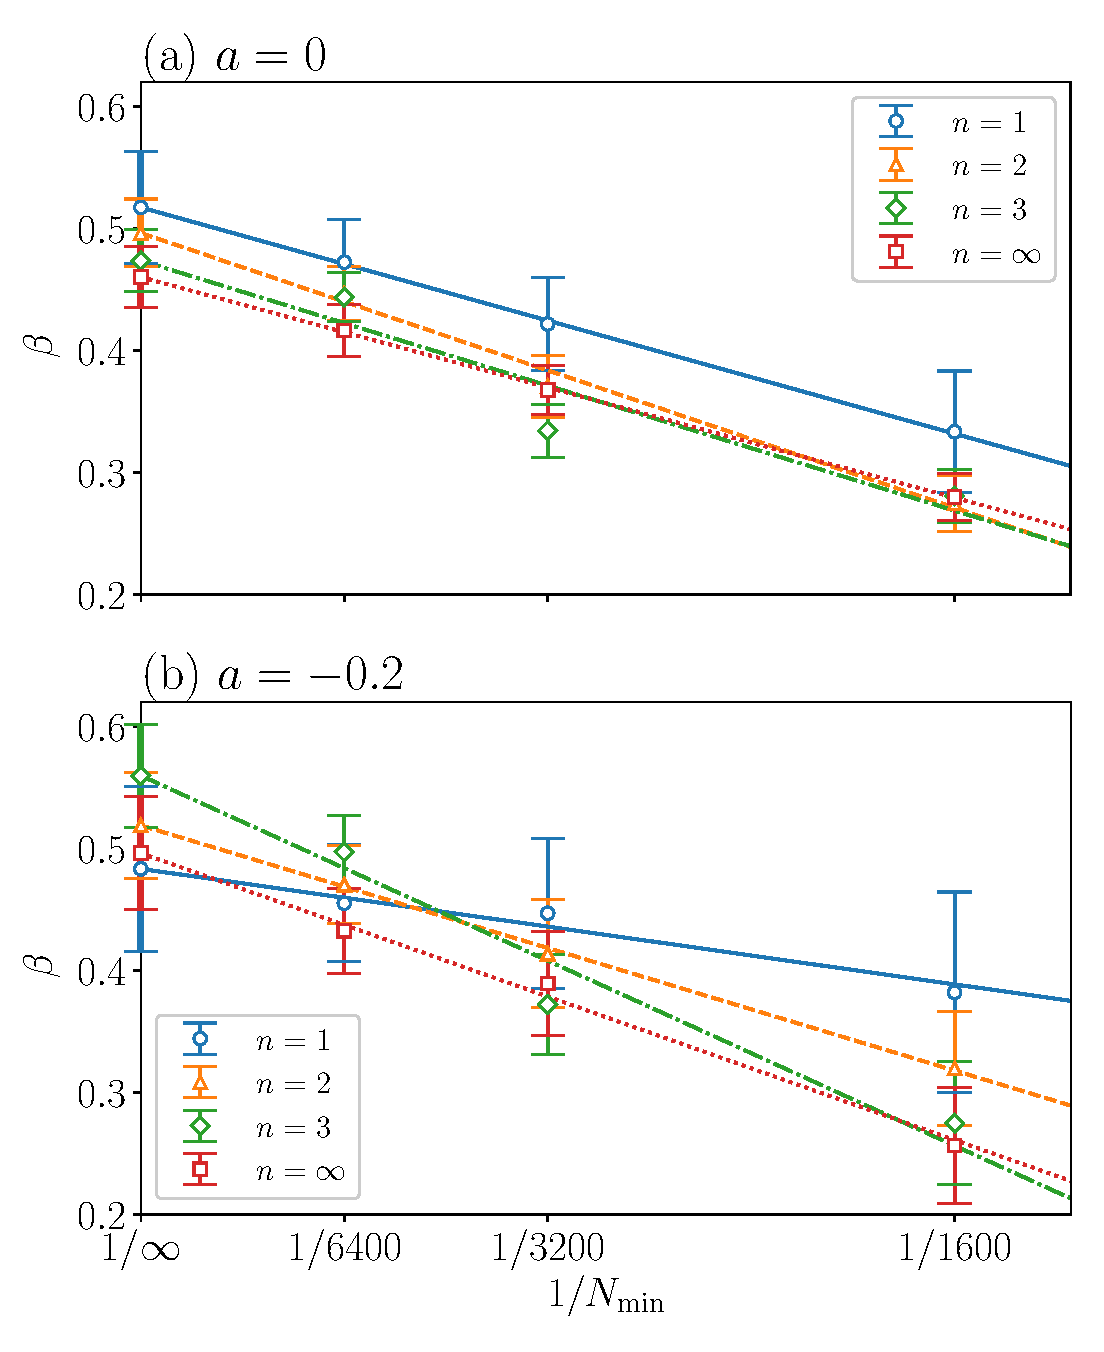
\includegraphics[width=8cm]{figs/beta_extrapolation.eps}
    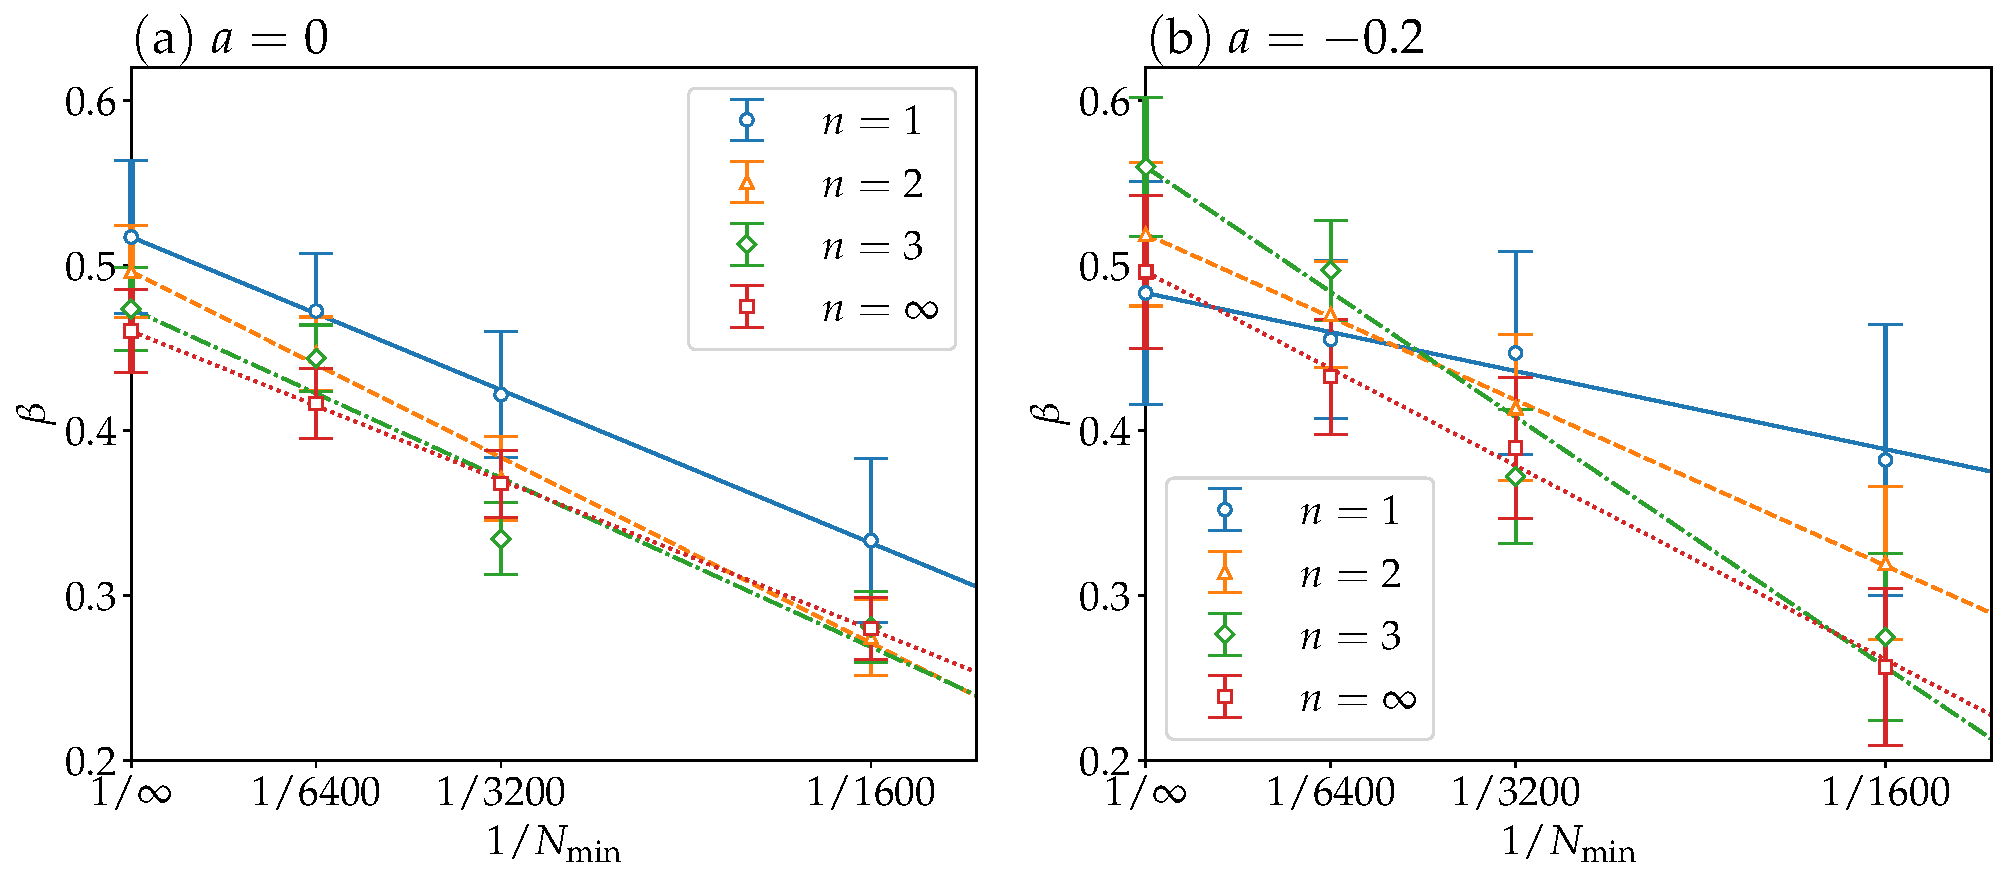
\includegraphics[width=\textwidth]{figs/beta_N_dep.pdf}
  \end{center}
  \caption{Graphs of $\beta$ as a function of $1/N_{\min}$
    for (a) $a=0$ and (b) $a=-0.2$ in Eq.~\eqref{eq:sw-model}.
    Critical exponents obtained by the finite-size scaling
    are shown with errorbars,
    %and their extrapolations are shown at $1/N_{\min}=1/\infty$,
%    which are calculated by the least square method.
    and the least square method gives the extrapolations
    at the left boundary of the panels.
    For each $a$, the resulting linear regression lines are drawn with the solid line for $n=1$,
    the dashed line for $n=2$, the dot-dashed line for $n=3$, and the dotted line for $n=\infty$.
  }
  \label{fig:ce_extrapolation}
\end{figure}

% By observing the computed parameters shown in Table \ref{table:parameter-estimate},
%we find that $\beta$ converge to
%\begin{align}
%  \beta\simeq\frac{1}{2},
%\end{align}
% \red{we find that $\beta$ tends to approach to $1/2$ as $N$ increases,}
% which is independent of $a$ and $n$, 
% unlike the coupled phase-oscillator on the all-to-all network.
%Table~\ref{table:critical-exponent} shows the comparison of critical exponents $\beta$
%for the all-to-all and a small-world network.
%\begin{table}
%  \begin{center}
%    \caption{
%    Comparison of critical exponent $\beta$ for the all-to-all and a small-world network.  
%    Here, (D) denotes a discontinuous transition.
%    All the values of $\beta$ shown in the all-to-all network are all theoretically calculated~\cite%{kuramoto1975,strogatz2000,chiba2015,daido2015,basnarkov2007,pazo2005,daido1990,crawford1995,%chiba2011,pikovsky2013}.
%    Because for $g_{\infty}(\omega)$ in the Kuramoto model,
%    there is some constant $r_{\mathrm{c}}>0$ such that $r-r_{\mathrm{c}}\sim(K-K_{\mathrm{c}})^{2/3}%$~\cite{basnarkov2007,pazo2005,daido1990},
%    we put parentheses to distinguish from other $\beta$.
%    We also note that values of $\beta$ shown in the small-world network are predicted
%    from the estimated values using the Bayesian scaling analysis, Table \ref%{table:parameter-estimate}.
%    }
%    \label{table:critical-exponent}
%    \begin{tabular}{c|ccc|ccc}\hline
%     & \multicolumn{3}{c|}{all-to-all} & \multicolumn{3}{c}{small-world} \\\cline{2-7}
%     & $a<0$ & $a=0$ & $0<a<1$ & $a<0$ & $a=0$ & $a>0$\\\hline\hline
%    $n=1$ & \multirow{3}{*}{\begin{tabular}{c}$1$\\\cite{crawford1995,chiba2011,pikovsky2013}\end%{tabular}} & $1/2$~\cite{kuramoto1975,strogatz2000,chiba2015} & \multirow{3}{*}{\begin{tabular}{c}%(D)\\\cite{crawford1995,chiba2011}\end{tabular}} & \multicolumn{2}{c}{\multirow{3}{*}{%{\LARGE$\frac{1}{2}$}}} & \multirow{3}{*}{\begin{tabular}{c}(D)\end{tabular}}\\
%    $n\geq 2$ &  & $1/(2n)$~\cite{daido2015} &  &  &  & \\
%    $n=\infty$ &  & $(2/3)$~\cite{basnarkov2007,pazo2005,daido1990} &  &  &  & \\\hline
%    %\begin{tabular}{c|ccc}\hline
%    %& \multicolumn{3}{c}{all-to-all} \\\cline{2-4}
%    %& $a<0$ & $a=0$ & $0<a<1$ \\\hline\hline
%    %$n=1$ & $1$ & $1/2$ & (D) \\
%    %$n\geq 2$ & $1$ & $1/(2n)$ & (D)\\
%    %$n=\infty$ & $1$ & $(2/3)$ & (D) \\\hline\hline
%    %& \multicolumn{3}{c}{small-world} \\\cline{2-4}
%    %& $a<0$ & $a=0$ & $a>0$\\\hline\hline
%    %$n=1$ & $1/2$ & $1/2$ & (D)\\
%    %$n\geq 2$ & $1/2$ & $1/2$ & (D)\\
%    %$n=\infty$ & $1/2$ & $1/2$ & (D)\\\hline
%    \end{tabular}
%  \end{center}
%\end{table}

% We notice that the critical exponent $\bar{\nu}$ obtained in \cite{hong2002},
% claiming that $\bar{\nu}\simeq2$ for $(a,n)=(0,1)$, is different from ours, $\bar{\nu}\simeq 5/2$.
% They first find the best fit $\beta/\bar{\nu}$ and $K_{\mathrm{c}}$
% at which $r_{N}(K)N^{\beta/\bar{\nu}}$ crosses at $K=K_{\mathrm{c}}$
% by varying the system size $N$.
% Then they use the following formula,
% \begin{align}
%   \log\left[\frac{\diff r_{N}}{\diff K}(K_{\mathrm{c}})\right]=\frac{1-\beta}{\bar{\nu}}\log N+\mathrm{const.},
% \end{align}
% which is calculated by taking the derivative of (\ref{eq:finite-size}) with respect to $K$,
% and they calculate $(1-\beta)/\bar{\nu}$ by computing the slope of $\log[\frac{\diff r_{N}}{\diff K}(K_{\mathrm{c}})]$ with respect to $\log N$.
% However this method has a disadvantage
% that the estimated critical point $K_{\mathrm{c}}$ is needed for calculating $(1-\beta)/\bar{\nu}$.
% Also, this method does not take into account the numerical results $r_{N}(K)$ for $K\ne K_{\mathrm{c}}$.
% %Therefore, our estimation of the critical exponents, where we use the Bayesian scaling analysis,
% %is more reliable than the one obtained in \cite{hong2002}.
% %revise
% %We believe that our estimation of the critical exponents is more reliable
% %because it uses the Bayesian scaling analysis which overcomes these disadvantages.
% \red{Our estimation of the critical exponents is more reliable than \cite{hong2002}
% because our Bayesian scaling analysis~\cite{harada2011,harada2015} simultaneously estimates a critical point and critical exponents without an explicit scaling function.}

The value $\bar{\nu}\simeq 5/2$ is not in agreement
with the value $\bar{\nu}\simeq 2$ previously reported
for $(a,n)=(0,1)$ \cite{hong2002}.
We suppose that the discrepancy comes from the method
to compute the critical exponents.
In the literature, the authors used the fact
that $r_{N}(K)N^{\beta/\bar{\nu}}$ takes a constant value
irrespective of $N$ at the critical point $K=K_{\rm c}$
(See Eq.~\eqref{eq:finite-size}). Using this fact,
they first find the best fit values of $\beta/\bar{\nu}$ and $K_{\rm c}$
by varying the system size $N$. One more equation is obtained
by derivating the finite-size scaling, Eq.~\eqref{eq:finite-size},
which produces
\begin{equation}
  \log\left[ \frac{\diff r_{N}}{\diff K}(K_{\mathrm{c}}) \right]
  = \dfrac{1-\beta}{\bar{\nu}} \log N + \mathrm{const.}
\end{equation}
Plotting the left-hand side as a function of $\log N$,
one has the slope $(1-\beta)/\bar{\nu}$.
A remarkable disadvantage of this method is that
the estimation relies on high precision of $r_{N}(K)$
around the critical point $K=K_{\rm c}$,
while the Bayesian scaling analysis uses $r_{N}(K)$
in a wider interval of $(K-K_{\rm c})N^{1/\bar{\nu}}$
and provides persistence against fluctuation.
We, therefore, believe that $\bar{\nu}\simeq 5/2$
obtained by the Bayesian scaling analysis is more reliable.


\subsection{Discontinuity of transition}

% \red{In some Kinetic models, the existence of quasi-stable states and their switch at a transition point is a reason for the discontinuous transition. If the quasi-stable states exits, we can observe an order parameter's hysteresis for different initial conditions.
% Here,}
% we check the hysteresis of (\ref{eq:sw-model}) with $a=0.5$
% by taking two different types of initial phases $\{\theta_{i}\}_{i=1}^{N}$:
% (i) We start with the random initial phases $\{\theta_{i}\}_{i=1}^{N}$ at $K=K_{\mathrm{start}}$,
% and the final phases at $t=500$ is used as the initial phases at the successive value of $K$ in the increasing direction.
% We call this process the ``forward'' process, and $r_{N}^{(\mathrm{forward})}(K)$ denotes its order parameter.
% (ii) Contrary to the ``forward'' process, we start with the random initial phases $\{\theta_{i}\}_{i=1}^{N}$ at $K=K_{\mathrm{end}}$,
% and the final phases at $t=500$ is used as the initial phases at the successive value of $K$ in the decreasing direction.
% We call this process the ``backward'' process, and $r_{N}^{(\mathrm{backward})}(K)$ denotes its order parameter.
% We have executed the numerical simulations of (\ref{eq:sw-model})
% for $a=0,-0.2$, and $0.5$, and $n=1,2,3$, and $\infty$, and $N=25600$ with two different initial phases as shown above,
% and confirmed that there exists a hysteresis only for $a=0.5$ regardless of $n$.
% \red{
% We remark that we have checked that $t=500$ is enough for the systems to pass the transition period,
% and the further simulation $t\geq500$ does not affect the hysterisis.
% }
% See Fig.~\ref{fig:hysteresis} for an example of a hysteresis with $(a,n)=(0.5,1)$.
% We therefore conclude that the coupled phase-oscillator model (\ref{eq:sw-model})
% shows a discontinuous transition for $a=0.5$.

\begin{figure}[t]
  \begin{center}
    % 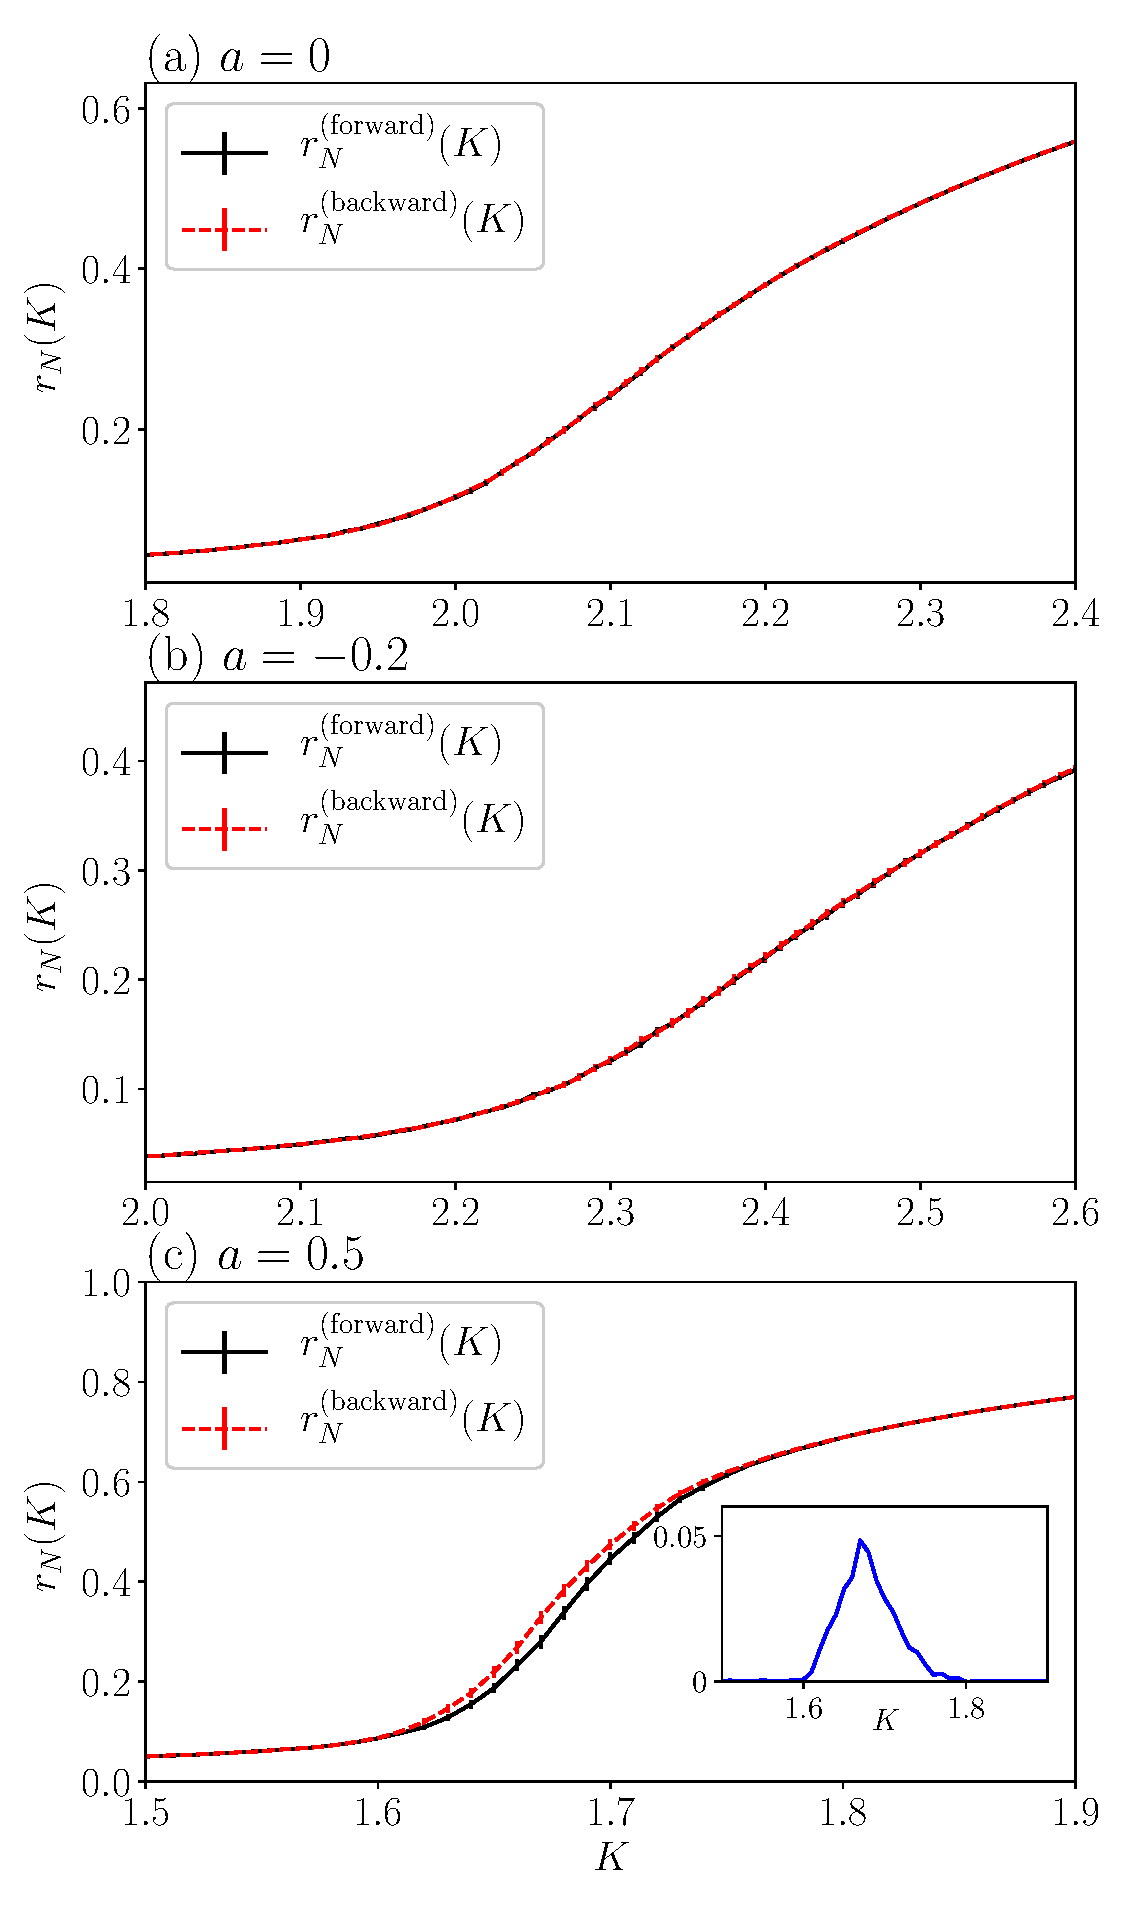
\includegraphics[width=8cm]{figs/hysteresis.eps}
    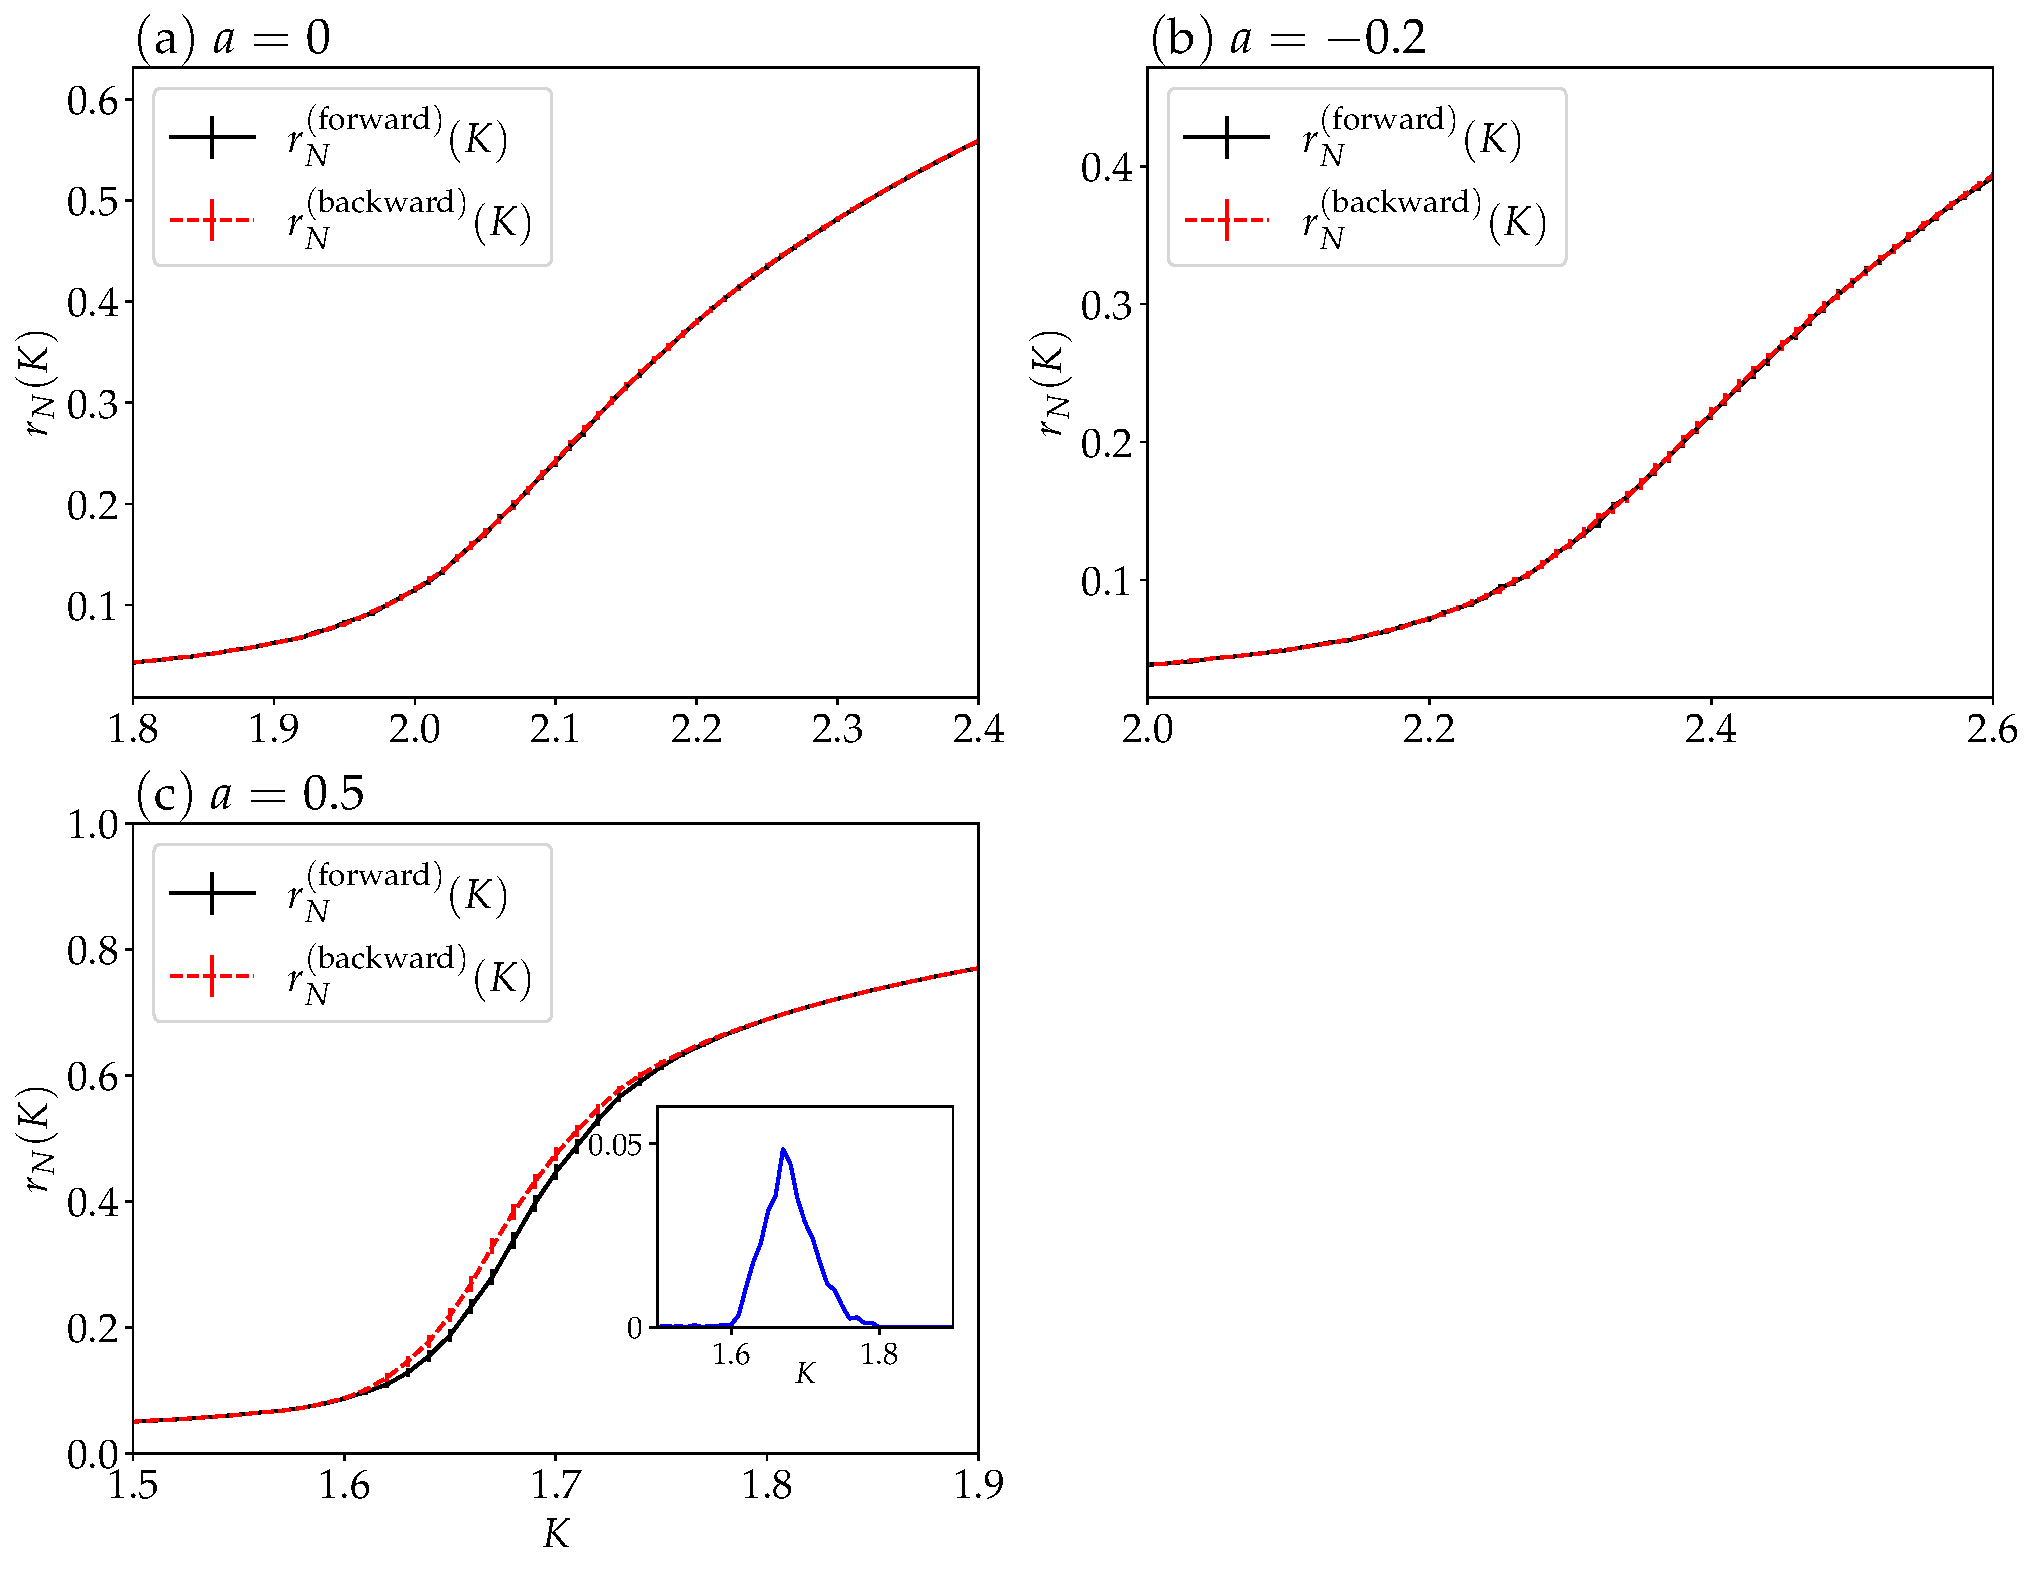
\includegraphics[width=\textwidth]{figs/check_hysteresis.pdf}
    \caption{
      Graphs of $r_{N}(K)$ and its errorbar of \eqref{eq:sw-model}
      for (a) $(a,n)=(0,1)$, (b) $(a,n)=(-0.2,1)$, and (c) $(a,n)=(0.5,1)$
      with two different types of initial phases,
      where we set the number of oscillators $N=25600$.
      We see that, only in (c), $r_{N}(K)$ takes a different value depending on the choice of the initial phases
      around $K\in(1.6,1.8)$.
      The inset in (c) shows the graph of $r_{N}^{(\mathrm{backward})}(K)-r_{N}^{(\mathrm{forward})}(K)$.
    }
    \label{fig:hysteresis}
  \end{center}
\end{figure}

In the all-to-all interaction
a positive $a$ induces discontinuity of the synchronization transition
\cite{chiba2011}.
We reveal that the transition is discontinuous
also in a small-world network.
The discontinuity appears as a result of a subcritical transition,
and a subcritical transition has metastability:
A partially synchronized state is stable in addition to
a stable nonsynchronized state for a fixed $K$ close to the critical point.
The metastability implies that the final state depends on
choice of the initial state,
and the dependency is extracted by observing hysteresis.

Fixing $a=0.5$, we check existence of the hysteresis
by preparing two sets of the initial phases $\{\theta_{i}\}_{i=1}^{N}$
for each $K$:
(i) We start from $K=K_{\mathrm{start}}$,
where $K_{\rm start}$ is sufficiently smaller than the critical value $K_{\rm c}$,
and the initial phases $\{\theta_{i}\}_{i=1}^{N}$ are randomly drawn
from the interval $[0,2\pi)$.
At a certain value of $K$, the final phases at $t=500$ is used
as the initial phases at the successive value $K+\Delta K$
in the increasing direction.
The increase of $K$ is continued up to $K=K_{\rm end}$,
where $K_{\rm end}$ is sufficiently larger than the critical value $K_{\rm c}$.
%    
% We start with the random initial phases $\{\theta_{i}\}_{i=1}^{N}$ at $K=K_{\mathrm{start}}$,
% \blue{where $K_{\rm start}$ is sufficiently smaller than the critical value $K_{\rm c}$.}
% The final phases at $t=500$ is used as the initial phases at the successive value $K=K_{\rm start}+\Delta K$ in the increasing direction.
We call the process (i) the ``forward'' process, and $r_{N}^{(\mathrm{forward})}(K)$ denotes its order parameter.
(ii) Contrary to the ``forward'' process,
we start with the random initial phases $\{\theta_{i}\}_{i=1}^{N}$
at $K=K_{\mathrm{end}}$
and decrease $K$ up to $K=K_{\rm start}$
following the same procedure with the ``forward'' process.
% and the final phases at $t=500$ is used as the initial phases at the successive value of $K=K_{\rm end}-\Delta K$ in the decreasing direction.
% \blue{This process is continued up to $K=K_{\rm start}$.}
We call this process the ``backward'' process, and $r_{N}^{(\mathrm{backward})}(K)$ denotes its order parameter.
We have executed the numerical simulations of Eq.~\eqref{eq:sw-model}
for $a=0,-0.2$, and $0.5$, and $n=1,2,3$, and $\infty$.
For the system size $N=25600$,
the hysteresis appears only for $a=0.5$ regardless of $n$
as exampled in Fig.~\ref{fig:hysteresis} for $n=1$.
% \red{
% We remark that we have checked that $t=500$ is enough for the systems to pass the transition period,
% and the further simulation $t\geq500$ does not affect the hysterisis.
% }
%   See Fig.~\ref{fig:hysteresis} for an example of a hysteresis with $(a,n)=(0.5,1)$.
We have checked that $t=500$ is sufficiently long
to pass the transient period,
and simulations up to $t=800$ do not affect the hysteresis.
We therefore conclude that the system represented by Eq.~\eqref{eq:sw-model}
shows a discontinuous transition for $a=0.5$ as the all-to-all interaction case.


\section{Small-world network and noise}
\label{sec:SW-noise}

We discuss similarity between systems on small-world networks
and noise systems.
For simplicity, we consider the Kuramoto model $(a=0)$ for a while.
The steady state in the Kuramoto model is
proportional to $\delta(\omega-Kr\sin\theta)$
in the synchronized regime
of $\omega$ \cite{strogatz2000,fonseca2018},
where $\delta$ is the Dirac's delta function.
The $\delta$ function with the integration over $\omega$
and symmetry of the natural frequency distribution
yield the self-consistent equation of the order parameter $r$ as
\begin{align}
  r=Kr\int_{-\pi/2}^{\pi/2}g_{n}(Kr\sin\theta)\cos^{2}\theta\diff\theta.
  \label{eq:self-consistent}
\end{align}
The order parameter $r$ is sufficiently small around the critical point
and we perform the Maclaurin expansion of $g_{n}$.
The leading order of the expansion, which is of $O(r)$,
determines the celebrated critical point $K_{\rm c}=2/[\pi g_{n}(0)]$.
The partially synchronized branch is obtained
by balancing the second leading order of $O(r^{2n+1})$
with the first leading order of $O(r(K-K_{\rm c}))$,
and the balance results to $r\propto (K-K_{\rm c})^{1/(2n)}$.
We then obtain the critical exponent $\beta=1/(2n)$.

To the contrary, on a small-world network,
a steady state is not written in the form of the $\delta$ function
and the synchronized oscillators are still ``noisy''
as shown in Fig.~\ref{fig:all-sw-scatter}.
The synchronized oscillators no longer capture
the flatness of $g_{n}(\omega)$ around $\omega=0$,
and the critical exponent $\beta$ falls into the classical value $1/2$
regardless of natural frequency distribution $g_{n}(\omega)$
as a noisy system \cite{sakaguchi1988}.

Moreover, in the model having the nonvanishing second harmonics
of the coupling function with $a<0$,
the noise recovers $\beta=1/2$ \cite{crawford1995}
whereas no noise system gives $\beta=1$ \cite{daido1994}.
The universality of $\beta=1/2$ observed in systems on small-world networks
is therefore very similar to the one in noisy systems.

\begin{figure}[t]
    \centering
    % \includegraphics[width=8cm]{figs/all-sw-scatter.eps}
    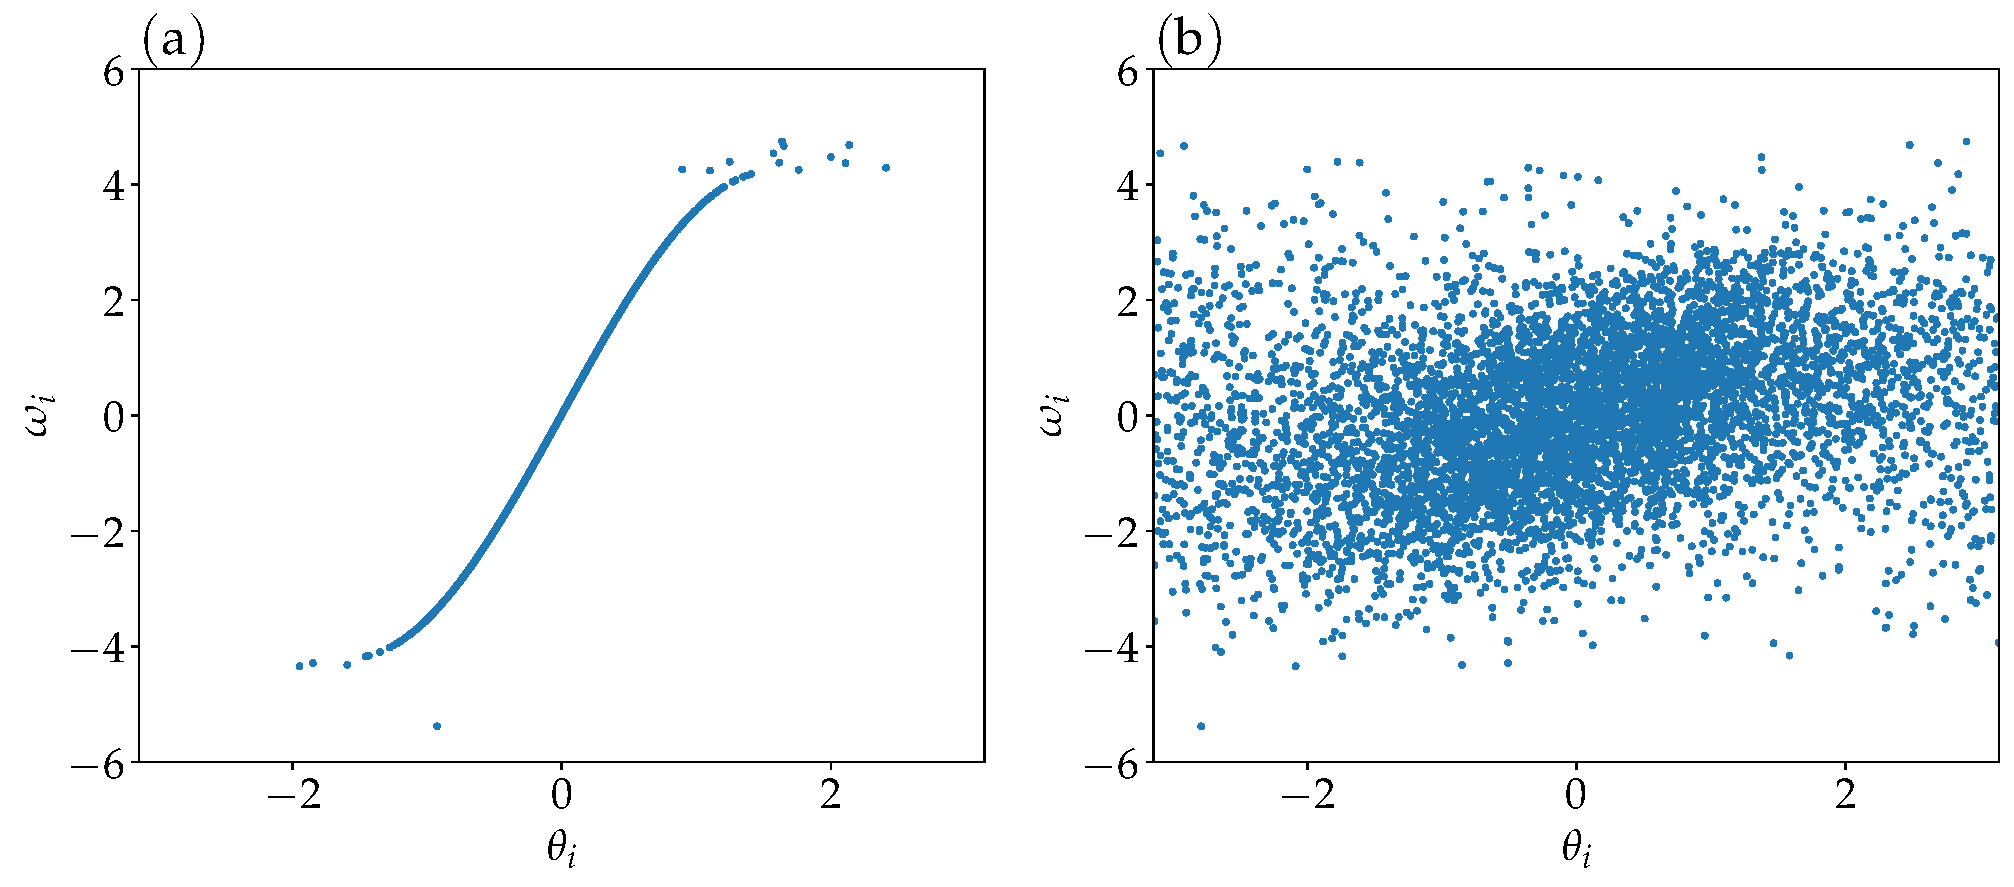
\includegraphics[width=\textwidth]{figs/all_sw_snap.pdf}
    \caption{
      Snap shots of oscillators on the $(\theta_{i},\omega_{i})$ plane
      at $t=500$.
      (a) The all-to-all network.  (b) A small-world network.
      The system size $N=6400$. The coupling constant $K=4.5$.
      $(a,n)=(0,1)$.
    % and integrate the differential equation (\ref{eq:sw-model}) up to $t=500$ with the time step $\delta t=0.1$.
    }
    \label{fig:all-sw-scatter}
\end{figure}



\section{Summary and Discussions}
\label{sec:conclusion}
We calculated the critical exponents $\beta$ and $\bar{\nu}$
for coupled phase-oscillator models on small-world networks
%in (\ref{eq:sw-model})
by using the finite-size scaling method.
We set the coupling function as $f_{a}(\theta)=\sin\theta+a\sin2\theta$, and the natural frequency distribution
as $g_{n}(\omega)$ defined in Eq.~\eqref{eq:g_n},
and we studied the $(a,n)$-dependency of the critical exponents.
%As summarized in Table~\ref{table:critical-exponent},
Our numerical results suggest $\beta=1/2$ and $\bar{\nu}=5/2$
for all $g_{n}(\omega)$ and coupling function $f_{a}(\theta)$ with $a=0$ and $-0.2$.
%which means that all such systems are in the same universality class.
%which share the same critical exponents for the Kuramto model with $n=1$ \cite{hong2007}.
%natural frequency distribution~.
This universality shows a sharp contrast with the all-to-all interaction case,
which has various values of $\beta$ depending on the coupling function and the natural frequency distribution.
A possible explanation of the source of contrast
can be found in the number of links of considering networks:
our small-world networks has $O(N)$ links,
while the all-to-all interaction have $O(N^{2})$ links.
% Remarking that 
% the coupled phase-oscillator models on a small-world network with $O(N^{2})$ \blue{links}~\cite{chiba2018,medvedev2014}
% shares the same critical exponent as the Kuramoto model, whose network also has $O(N^{2})$ \blue{links},
% we believe that this contrast comes from the number of \blue{links} of networks.
We have also found that the model, Eq.~\eqref{eq:sw-model},
shows a discontinuous transition for $a=0.5$.
%As can be seen in Table~\ref{table:critical-exponent},
%This discontinuity is consistent
%with the one with the coupled phase-oscillator model on the all-to-all network for $0<a<1$.
The (dis)continuity is a weaker property than the values of the critical exponents,
and it is shared between the two types of networks:
networks with $O(N)$ links and $O(N^{2})$ links.

% \red{
% Here, we discuss the difference of the critical exponent $\beta$ in the coupled phase-oscillator models on the all-to-all network and a small-world network.
% In the Kuramoto model, the steady state of the oscillators is written
% in the form of $\delta$ function~\cite{strogatz2000,fonseca2018}.
% See Fig.~\ref{fig:all-sw-scatter}(a) for the numerical simulation of the Kuramoto model.
% This steady state yields the famous Kuramoto self-consistent equation~\cite{strogatz2000,fonseca2018}, which reads
% \begin{align}
%     r=Kr\int_{-\pi/2}^{\pi/2}g_{n}(Kr\sin\theta)\cos^{2}\theta\diff\theta,
%     \label{eq:self-consistent}
% \end{align}
% and we get $r\propto(K-K_{\mathrm{c}})^{1/(2n)}$ by using the Maclaurin form  (\ref{eq:maclaurin}).
% On the contrary, in the coupled phase-oscillator models on the small-world network,
% the steady state cannot be written in the form of $\delta$ function
% due to the complexity of the network.
% As can be seen in Fig.~\ref{fig:all-sw-scatter}(b),
% the synchroized oscillators somehow distributed in a ``noisy'' way, 
% which is quite different from the Kuramoto model.
% Hence they no longer capture the flatness of $g_{n}(\omega)$,
% and the critical exponent $\beta$ falls into the classical value $1/2$
% regardless of natural frequency distribution $g_{n}(\omega)$.
% }




We end this chapter commenting on two future works.
Firstly,
%we mainly focused on the dependence of critical exponents
%of the natural frequency distribution, and we picked representative points of $a$ from around $a=0$
%to check universality in the coupled phase-oscillator models on a small-world network.
we picked up two representative points of $a$ from a neighborhood of $a=0$
to investigate universality of the critical exponents.
Studying a global phase diagram on the $(K,a)$-plane is a subject for future researches.
Secondly, we note universal value $\beta=1/2$ in the Kuramoto model
which is recovered by adding noise regardless of the natural
frequency distribution \cite{sakaguchi1988}.
A small-world network may play a role of noise due to
inhomogeneous couplings,
and another work to do is to make a bridge between a noisy Kuramoto model
and a model on a small-world network.

% Secondly, we note a relationship with the noisy Kuramoto model.
% In the Kuramoto model, the value of $\beta$ depends on the natural frequency distribution, 
% but by adding some noises, $\beta=1/2$ is consistent regardless of the natural frequency distribution~\cite{sakaguchi1988}.
% This value is similar to the one in the coupled phase-oscillator models on a small-world network
% with a reasonable choice of the $1/N$ extrapolation performed in Fig.~\ref{fig:ce_extrapolation}.
% These coincidence thus suggests
% %that using the small-world network for the coupled phase-oscillator model
% %gives the same effect as applying noises to the coupled phase-oscillator on the all-to-all network.
% %This relationship needs to be investigated.
% introducing the small-world network plays a similar role with applying noises
% because of its inhomogeneous couplings.



%Thirdly, in addition to the critical exponent $\beta$,
%there are still other critical exponents to calculate,
%$\gamma$ and $\delta$ concerning with response for instance.
%Once we obtain three critical exponents,
%we can check if the Widom equality $\gamma=\beta(\delta-1)$ holds.
%For the Kuramoto model, the Widom equality is obtained
%by analyzing the self-consistent equation with respect to $r$~\cite{daido2015}.
%However, we cannot derive the self-consistent equation for the coupled phase-oscillator model
%on the small-world network,
%and it is not obvious if the Widom equality holds.

%Fourthly, it remains to clarify $\alpha$-dependence of the critical exponent $\beta$
%in coupled phase-oscillator models with $O(N^{\alpha})$-edge networks ($1<\alpha<2$).
%This $\alpha$-dependence may make a bridge to the gap between  $\alpha=2$ and $1$,
%which has been revealed in this paper.

%Finally,
%since we numerically obtained $\beta$,
%it is natural to check the value theoretically.
%To investigate critical phenomena in the model (\ref{eq:sw-model}),
%one has to consider the large population limit $N\to\infty$,
%but to the best of our knowledge,
%we do not have a tool for taking the large population limit
%with network of $O(N)$ \blue{links}.
%It is challenging to attack this problem.

%3???4????????
%Thirdly,
%in this paper we used small-world networks with $O(N)$ \blue{links},
%but other complex networks are to be studied.
%For example,
%a coupled phase-oscillator model on a scale-free network is studied in \cite{yoon2015} by using the %Ott-Antonsen ansatz,
%and the critical exponent $\beta$ explicitly depends on the degree distribution of the scale-free %network.
%Coupled phase-oscillator models on other networks,
%such as a random sparse network, and $d$-dimensional lattice networks,
%have been obtained by the finite-size scaling method~\cite{juhasz2019,hong2007}.
%The theoretical derivation of the values of $\beta$
%for the models on these networks is to be investigated.
%Finally,
%the coupled phase-oscillator models with $O(N^{\alpha})$-edge networks ($1<\alpha<2$)
%should also be investigated.
%It remains to clarify $\alpha$-dependence of the critical exponent $\beta$,
%which may depend on $\alpha$ as revealed in this paper.


% \appendix
